%#!platex jou.tex
\chapter{\texorpdfstring \LaTeX {LaTeX}の応用}\chaplab{ouyou}

\begin{abstract}
以下に示すコマンドなどはレポートや論文には必要
不可欠という程の要素ではありませんが,%この
%ような機能もあるという程度でご覧ください.
いざという時に役に立つかもしれませんので,簡単に説明しておきます.
\end{abstract}


\section{ページレイアウトの簡単な設定}
\zindind{ページ}{レイアウト}


\subsection{版面のレイアウト}\seclab{layout}

\KY{版面}のレイアウトを行う場合にはそれぞれの
長さに対して直接値を代入する方法があります.
{\LaTeX}で一般的に設定できる版面を調節する
長さは\figref{pagelayout}の通りです.
\begin{figure}[p]
 \begin{center}
  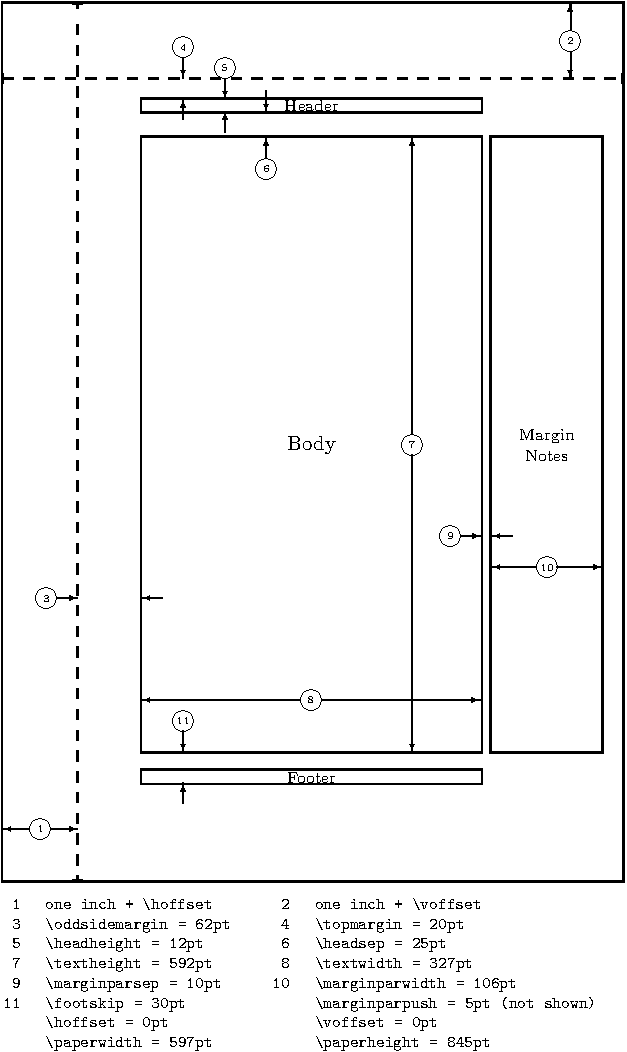
\includegraphics[width=.8\textwidth]{images/mylayout}
  \caption{版面のレイアウトに使用できる長さ}\figlab{pagelayout}
 \end{center}
\end{figure}
\indindz{ファイル}{クラス}%
このような版面を視覚的に確認するには\Y{layout}パ
ッケージが使えます.このパッケージは使用されている%
クラスファイルから版面のレイアウトを出力します.
使用方法は\env{document}環境中で \C{layout} 命令を
使うだけです.

\begin{Prob}
\Y{layout}パッケージを使って,特定のクラスファイルの標準的
なページレイアウトがどのようになっているかを,次のような
ファイルをタイプセットする事により確認してください.

\begin{InTeX}
\documentclass{jsarticle}
\usepackage{layout}
\begin{document}
\layout
\end{document}
\end{InTeX}

\cls{jsarticle}以外にも \Cls{jsbook} や \Cls{jbook} 等でも
確認してみてください.
\end{Prob}


\index{用紙}
まずはページ全体の\Z{余白}に関する長さです.\zindind{ページ}{の余白}
\begin{description}
 \item[\Cmd{voffset}] \zindind{用紙}{の空白}
 横組みにおいて用紙の左上の部分に入れる縦方向の余白.
 この値を0にしてもすでに1インチ分の余白が挿入されています.
 本当に用紙の左上端から使うならば \cmd{voffset}を
 \qu{\str{-1in}}に設定します.

 \item[\Cmd{hoffset}] 
 横組みにおいて用紙の左上の部分に入れる横方向の余白.
 縦方向と同じようにすでに1インチ分の余白が挿入されています.

 \item[\Cmd{oddsidemargin}]
ページが奇数のときに挿入される左側の余白.
文書クラスオプションに\Option{oneside}を
使っていると全てのページに \cmd{oddsidemargin}が
挿入されます.

 \item[\Cmd{evensidemargin}] 
ページが偶数のときに挿入される左側の余白.
文書クラスオプションに\Option{twoside}を
使っているときだけ有効で\Option{oneside}では
意味がありません.
\end{description}

ヘッダの設定に関する長さです.
\begin{description}
\item[\Cmd{topmargin}] 
\cmd{voffset}とヘッダの間隔です.
\item[\Cmd{headheight}]
ヘッダの高さです.\indindz{高さ}{ヘッダの}%
\item[\Cmd{headsep}]
ヘッダと本文領域の間隔です.
\item[\Cmd{footskip}]
フッタ下部と本文領域の最下部との間隔です.
\end{description}

本文領域や傍注領域に関わる長さです.
\begin{description}
\item[\Cmd{textheight}]\indindz{高さ}{本文領域の}%
 本文領域の高さです.ヘッダやフッタの高さは含まれません.
 \item[\Cmd{textwidth}]
 本文領域の幅です.\indindz{幅}{本文の}%
 \item[\Cmd{marginparwidth}]
  傍注の幅です.\indindz{幅}{傍注の}%
 \item[\Cmd{marginparpush}]
 傍注と傍注のあいだの縦方向の長さです.
 \item[\Cmd{marginparsep}]
 傍注と本文領域との間隔です.
 \item[\Cmd{columnsep}]
 2段組以上での段と段の間隔です.
 \item[\Cmd{columnseprule}]
 2段組以上での段と段のあいだに入る罫線です.\indindz{罫線}{2段組での}
\end{description}
通常ここで紹介した長さはクラスファイル側
でフォントサイズやクラスオプションに応じ
て適切に設定されますので徒に変更しないでください.\zindind{ページ}{の行数}
相手先の都合で\yo{1行何文字1ページ何行}
のような設定などをしなければならないときは無理やり
次のようにする事もできます.

\begin{InTeX}
\setlength{\textwidth}{33zw}
\setlength{\textheight}{40\baselineskip}
\end{InTeX}



\subsection{簡単なページレイアウト\zdash \Y{geometry}}
\zindind{版面}{の設定}%
\indindz{余白}{上下左右の}%

例えば,「上下左右の余白を 2\,cm とし,残りの領域は本文に使い,
\Z{フッター}と\Z{ヘッダー}は本文の領域の高さに含める」という
ページレイアウトにしたければ,大雑把には次のような設定をする
事になります.
\begin{eqnarray*}
 \begin{aligned}
 \cmd{voffset}        & = -0.54\,\mathrm{cm} \\
 \cmd{hoffset}        & = -0.54\,\mathrm{cm} \\
 \cmd{evensidemargin} & = 0\,\mathrm{cm} \\ 
 \cmd{ossdidemargin}  & = 0\,\mathrm{cm} \\
 \cmd{textheight} 
   & = \cmd{paperheight} - 4\,\mathrm{cm} - \cmd{topmargin} \\
   & - \cmd{headheight} - \cmd{headsep} - \cmd{footskip}  \\
 \cmd{textwidth}   & = \cmd{paperwidth} - 4\,\mathrm{cm}  
 \end{aligned}
\end{eqnarray*}
これにより,\LaTeX では次のような設定をする事になります.

\begin{InTeX}
\setlength   \voffset        {-1in}% \voffset の設定
\addtolength \voffset        {2cm}
\setlength   \hoffset        {-1in}% \hoffset の設定
\addtolength \hoffset        {2cm}
\setlength   \textheight     {\paperheight}% \textheight の設定
\addtolength \textheight     {-4cm}
\addtolength \textheight     {-\topmargin}
\addtolength \textheight     {-\headheight}
\addtolength \textheight     {-\headsep}
\addtolength \textheight     {-\footskip}
\setlength   \textwidth      {\paperwidth}% \textwidth の設定
\addtolength \textwidth      {-4cm}
\setlength   \evensidemargin {0pt}% 偶数ページマージン
\setlength   \oddsidemargin  {\evensidemargin}% 奇数ページマージン
\setlength   \fullwidth      {\textwidth} 
\end{InTeX}

\indindz{印刷}{両面}%
しかし,\Z{両面印刷}をするとか,ヘッダーやフッターの高さを含む等の
調整が絡んでくると,少々入り組んだ設定になってしまいます.
そこで,もう少し簡単に版面の設定をしたいならば\Hito{梅木}{秀雄}
の作成した\sty{geometry}を使うのが良いでしょう.\Y{geometry}
パッケージは非常に多機能で,その全てを本書で紹介する事はできません
が,初学者がもっとも苦労し,様々な問題に直面する事が多いように見受けら
れますので,なるべく詳細に解説します.

使い方は非常に簡単で,プリアンブルで\Y{geometry}パッケージをオプション付
きで読み込むだけです.

\begin{InTeX}
\usepackage[margin=2cm]{geometry}
\end{InTeX}

上記のようにすると文章領域の上下左右の余白を 2\,cm に設定します
\footnote{用紙にはヘッダ,フッタ,傍注がありますから,これらの領域を除い
た文面の余白が 2\,cmという事になります.}.

他には \Y{geometry} パッケージを読み込んだ後に \C{geometry} コマンドを
使う方法です.これはプリアンブルのみで使う事ができます.

\begin{InTeX}
\usepackage[a5paper]{geometry} 
\geometry{hmargin={3cm,0.8in},height=8in}
\geometry{height=10in}
\end{InTeX}

\Y{geometry}パッケージは\Y{calc}パッケージにも対応していますので,
次のような記述も可能です.

\begin{InTeX}
\usepackage{calc}
\usepackage[textheight=20\baselineskip+10pt]{geometry}
\end{InTeX}

\Y{jsclasses}に含まれる,\Cls{jsbook}クラスを用いている場合
は \C{fullwidth} を \C{textwidth} に設定するのが良い時があります.

\begin{InTeX}
\setlength \fullwidth{\textwidth}
\end{InTeX}

以下に\Y{geometry}のパッケージオプションを挙げます.
パッケージオプションは基本的には \C{geometry} 命令の中で使うことができま
す.

\newcommand*\twoargs[2]{\texttt{\lb}\va{#1}\str,\va{#2}\texttt{\rb}}
\newcommand*\threeargs[3]{\texttt{\lb}\va{#1}\str,\va{#2}%
  \str,\va{#3}\texttt{\rb}}

\paragraph{用紙サイズ}

\begin{description}
 \item[既定のサイズ]
\zindind{用紙}{の既定のサイズ}
  \Optionlist{a0paper,a1paper,a2paper,a3paper,a4paper,a5paper,a6paper,%
  b0paper,b1paper,b2paper,b3paper,b4paper,b5paper,b6paper,%
  letterpaper,executivepaper,legalpaper,screen}.
  \option{screen} は 225\,mm $\times$ 180\,mm になります.
  \option{screen}は\option{centering} も併用すると便利です.
  `\str{paper=}\va{用紙サイズ}'と記述しても大丈夫です.
\item[\Option{paperwidth}] 
\zindind{用紙}{の幅}
  \Z{用紙}の幅を,\va{長さ}を指定して決めます.
  `\str{paperwidth=10cm}'のように使います.
\item[\Option{paperheight}]
\zindind{用紙}{の高さ}
  用紙の高さを,\va{長さ}を指定して決めます.
\item[\Option{papersize}]
  `\option{papersize}\str=\twoargs{幅}{高さ}'とするか,
  `\option{papersize}\str=\va{長さ}'とすれば \option{paperwidth}
  と\option{paperheight}を用いた事と等価になります.
\item[\Option{landscape}] 
  \Z{横置き}でページレイアウトを設定します.
\item[\Option{portrait}]
  \Z{縦置き}でページレイアウトを設定します.
\end{description}

\paragraph{本文のパラメータ}

\begin{description}
 \item[\Option{hscale}] 
  用紙の幅 (\C{paperwidth}) に対して本文領域が占める横幅の比率です.
  `\str{hscale=.8}' とすると `\str{width=.8\bs paperwidth}' と等価になりま
  す.標準は 0.7 です.
 \item[\Option{vscale}] 
  用紙の高さ (\C{paperheight}) に対して本文領域が占める高さの比率です.
  `\str{vscale=.8}' とすると `\str{height=.9\bs paperheight}' と等価になりま
  す.標準は 0.7 です.
 \item[\Option{scale}] 
  本文が幅と高さに関して用紙に対して占める比率を指定します.
  `\str{scale=}\twoargs{幅の比率}{高さの比率}'
   とするか`\str{scale=}\va{比率}'として使います.標準は 0.7 です.
 \item[\Option{width}/\Option{totalwidth}] 
\indindz{幅}{本文のトータルな}
  本文のトータルな幅を指定します.`\str{width=}\va{長さ}'とするか,
  `\str{totalwidth=}\va{長さ}'とします.
 \item[\Option{height}/\Option{totalheight}] 
\indindz{高さ}{本文のトータルな}
  本文のトータルな高さを指定します.`\str{height=}\va{長さ}'とするか,
  `\str{totalheight=}\va{長さ}'とします.
 \item[\Option{total}] 
  本文のトータルな幅と高さを指定します.
  `\str{total=}\twoargs{幅}{高さ}'とするか,
  `\str{total=}\va{長さ}'とします.
 \item[\Option{textwidth}] 
   文章領域となる \C{textwidth} の幅を指定します.
   `\str{textwidth=}\va{長さ}'とします.
 \item[\Option{textheight}]
   文章領域となる \C{textheight} の高さを指定します.
   `\str{textheight=}\va{長さ}'とします.
 \item[\Option{text}/\Option{body}]
  \C{textwidth} と \C{textheight} の両方を指定します.
  `\str{body=}\twoargs{幅}{高さ}'とするか`\str{text=}\va{長さ}'とします.
 \item[\Option{lines}]
  \cmd{textheight} を\Z{行数}によって決めます.`\str{lines=}\va{整数}'で指定
  します.
 \item[\Option{includehead}]
  トータルな本文の高さ\option{height}/\option{totalheight}にヘッダー
  (\C{headheight} と \C{headsep}) を含めるようにします.標準では無効です.
 \item[\Option{includefoot}]
  トータルな本文の高さ\option{height}/\option{totalheight}にフッター
  (\C{footskip}) を含めるようにします.標準では無効です.
 \item[\Option{includeheadfoot}]
  \option{includehead} と \option{includefoot} の両方を有効にします.
 \item[\Option{includemp}]
  トータルな本文の幅に\Z{傍注} (\C{marginparwidth} と \C{marginparsep}) も
  含めるようにします.\Option{marginparwidth}と\Option{marginparsep}オプ
  ションに依存しています.標準では無効です.
 \item[\Option{includeall}]
  \option{includeheadfoot} と \option{includemp} の両方を指定した事と等
  価です.
 \item[\Option{ignorehead}]
  トータルな本文の高さにヘッダーを含めないようにします.標準で有効です.
  `\str{includehead=false}'とするのと等価です.
 \item[\Option{ignorefoot}]
  トータルな本文の高さにフッターを含めないようにします.標準で有効です.
  `\str{includefoot=false}'とするのと等価です.
 \item[\Option{ignoreheadfoot}]
  \option{ignorehead} と \option{ignorefoot} の両方を指定した事と等価で
  す.
 \item[\Option{ignoremp}]
  トータルな本文の幅に傍注を含めないようにします.標準で有効です.
 \item[\Option{ignoreall}]
  \option{ignoreheadfoot} と \option{ignoremp} の両方を指定した事と等価
  です.
 \item[\Option{heightrounded}]
  本文の高さが行送りの倍数でない場合に,``\str{underfull vbox}''の警告を
  出さないように \C{textheight} を \va{\C{baselineskip} の整数倍 $+$
  \C{topskip}} にします.
 \item[\Option{hdivide}]
  左余白,文章の幅,右余白を指定します.`\str{hdivide=}%
  \threeargs{左余白}{文章幅}{右余白}'のように使います.
  このオプションは三つのうち二つだけ明確な時に,不定の一つを星`\str{*}'
  に置き換えて`\str{hdivide=\lb2cm,15cm,*\rb}'とできます.
 \item[\Option{vdivide}]
  \Z{上余白},文章の高さ,\Z{下余白}を指定します.`\str{vdivide=}%
  \threeargs{上余白}{文章幅}{下余白}'のように使います.
 \item[\Option{divide}]
  `\str{divide=}\threeargs{長さ\mbox{$_1$}}{長さ\mbox{$_2$}}{長さ
  \mbox{$_3$}}'とすると`\str{hdivide=}\threeargs{長さ\mbox{$_1$}}{長さ
  \mbox{$_2$}}{長さ\mbox{$_3$}}'と\str{vdivide=}\threeargs{長さ
  \mbox{$_1$}}{長さ\mbox{$_2$}}{長さ\mbox{$_3$}}'を指定した事と等価にな
  ります.
\end{description}

\paragraph{余白}

\begin{description}
 \item[\Option{left}/\Option{lmargin}/\Option{inner}]
 \zindind{用紙}{の左端}
 用紙の左端と本文領域(版面)とのあいだにある左余白を指定します.
 `\str{lmargin=}\va{長さ}'のように使います.両面印刷指定
 (\Option{twoside}) の場合は\Z{ノド}の長さを設定します.
 \item[\Option{right}/\Option{rmargin}/\Option{outer}]
 \zindind{用紙}{の右端}
 用紙の右端と本文領域とのあいだにある右余白を指定します.
 `\str{rmargin=}\va{長さ}'のように使います.両面印刷指定
 (\Option{twoside}) の場合は\Z{小口}の長さを設定します.
 \item[\Option{top}/\Option{tmargin}]
  用紙の上端と本文領域のとのあいだ(\Z{天})にある上余白を指定します.
 `\str{tmargin=}\va{長さ}'のように使います.
 \item[\Option{bottom}/\Option{bmargin}]
  用紙の下端と本文領域のとのあいだ(\Z{地})にある下余白を指定します.
 `\str{bmargin=}\va{長さ}'のように使います.
 \item[\Option{hmargin}]
  左右余白を指定します.`\str{hmargin=}\twoargs{左余白}{右余白}'とするか,
  `\str{hmargin=}\va{長さ}'とします.
 \item[\Option{vmargin}]
  上下余白を指定します.`\str{vmargin=}\twoargs{上余白}{下余白}'とするか,
  `\str{vmargin=}\va{長さ}'とします.
 \item[\Option{margin}]
  `\str{margin=}\twoargs{長さ\mbox{$_1$}}{長さ\mbox{$_2$}}'とすると,
  `\str{hmargin=}\twoargs{長さ\mbox{$_1$}}{長さ\mbox{$_2$}}'と
  `\str{vmargin=}\twoargs{長さ\mbox{$_1$}}{長さ\mbox{$_2$}}'を指定した
  事と等価になります.
 \item[\Option{hmarginratio}]
  左右余白の比率を指定します.`\str{hmarginration=}\va{左の比率\str:右の比率}'
  のようにコロンで区切ります.正の整数値で 100 以下である必要があります.
  片面印刷時 (\Option{oneside}) は $1:1$, 両面印刷時 (\Option{twoside})
  は $2:3$ が標準です.
  \item[\Option{vmarginratio}]
  用紙の上余白と下余白(\Z{天地})の比率を指定します.
 \item[\Option{marginratio}]
  `\str{marginratio=}\twoargs{左右の比率}{上下の比率}'とするか,
  `\str{marginration=}\va{比率}'とします.
 \item[\Option{hcentering}]
  `\str{hmarginration=1:1}'とした事と等価になります.
 \item[\Option{vcentering}]
  `\str{vmarginration=1:1}'とした事と等価になります.
 \item[\Option{centering}]
  `\str{marginration=1:1}'とした事と等価になります.
 \item[\Option{twoside}]
 \zindind{左右}{対称}
  \Z{両面印刷}時に文章領域(\Z{版面})が左右対称になるようにします.
 \item[\Option{asymmetric}]
 \zindind{左右}{非対称}
  両面印刷時に文章領域が左右非対称になるようにします.ただし,
  \option{bindingoffset}は考慮されます.
 \item[\Option{bindingoffset}]
  \zindind{文書}{を綴じる}
  \Z{片面印刷}時でも両面印刷時においても文書を綴じる背の部分の余白を
  指定します.`\str{bindingoffset=}\va{長さ}'として使います.
\end{description}

\paragraph{レイアウトパラメータの設定}

\LaTeX のページレイアウトにおけるパラメータを設定する事もできます.
%the options below specify \LaTeX\ native dimension and switches for page
%layout. See Figure~1. Note that unlike version~2.3, \option{nohead},
%\option{nofoot} and \option{noheadfoot} become overwritable, in other
%words, just shorthand for setting the corresponding \LaTeX\ dimensions
%(\cmd{headheight}, \cmd{headsep}, \cmd{footskip}) to 0\,pt.

\begin{description}
 \item[\Option{headheight}/\Option{head}] 
  `\str{head=}\va{長さ}'として \C{headheight} を設定します.
 \item[\Option{headsep}] 
  `\str{headsep=}\va{長さ}'として \C{headsep} を設定します.
 \item[\Option{footskip}/\Option{foot}] 
  `\str{foot=}\va{長さ}'として \C{footskip} を設定します.
 \item[\Option{nohead}] 
  ヘッダー無しの設定にします(\C{headheight} と \C{headsep} を 0\,pt
  にします).
 \item[\Option{nofoot}] 
  フッター無しの設定にします(\C{footskip} を 0\,ptにします).
 \item[\Option{noheadfoot}] 
  \option{nohead} と \option{nofoot} を指定した事と等価になります.
 \item[\Option{marginparwidth}/\Option{marginpar}] 
 \zindind{傍注}{の幅}
  `\str{marginpar=}\va{長さ}'として傍注の幅 \C{marginparwidth} を設定し
  ます.
 \item[\Option{marginparsep}]
 \zindind{傍注}{と本文の空き}
  `\str{marginparsep=}\va{長さ}'として傍注と本文の空き \C{marginparsep}
  を設定します. 
 \item[\Option{nomarginpar}]
  傍注無しの設定にします(\C{marginparwidth} と \C{marginparsep} を
  0\,pt にします).
 \item[\Option{columnsep}]
  `\str{columnsep=}\va{長さ}'として\Z{段間}の空き \C{columnsep} を設定します.
 \item[\Option{hoffset}]
  `\str{hoffset=}\va{長さ}'として \C{hoffset} を設定します.
 \item[\Option{voffset}]
  `\str{voffset=}\va{長さ}'として \C{voffset} を設定します.
 \item[\Option{offset}]
  `\str{offset=}\twoargs{水平方向のオフセット量}{垂直方向のオフセット量}'と
  するか`\str{offset=}\va{オフセット量}'として,\Z{オフセット}を指定します.
 \item[\Option{twocolumn}]
  2段組の設定にします.
 \item[\Option{twoside}]
  両面印刷用に傍注の位置を入れ換え,紙面を左右対称になるようにします.
 \item[\Option{textwidth}]
  `\str{textwidth=}\va{長さ}'として \C{textwidth} を直接指定します.
 \item[\Option{textheight}]
  `\str{textheight=}\va{長さ}'として \C{textheight} を直接指定します.
 \item[\Option{reversemp}/\Option{reversemarginpar}]
 傍注の位置を非標準の左側に出力するようにします.両面印刷時は
 \Z{見開き}の内側(小口)に設定します.
\end{description}

\paragraph{デバイスドライバ}

\begin{description}
 \item[\Option{dvips}] \Prog{dvips}用に用紙サイズ情報を設定します.
 \item[\Option{dvipdfm}] \Prog[dvipdfm]{\Dvipdfm}用に用紙サイズ情報を設
 定します.
 \item[\Option{pdftex}] \Prog[pdftex]{\PDFTeX},
 \Prog[pdflatex]{\PDFLaTeX}用に用紙サイズ情報を設定します.
\end{description}

\paragraph{その他}

\begin{description}
 \item[\Option{verbose}] 
  \Y{geometry}パッケージの処理内容を詳細に表示します.
 \item[\Option{showframe}] 
  ページレイアウトの設定を確認するために,1ページ目の本文領域,ヘッダー,
  フッターを枠で囲みます.
% \item[\Option{reset}] 
% \item[\Option{mag}] 
% \item[\Option{truedimen}] 
% \item[\Option{pass}] 
% \item[\Option{compat2}] 
\end{description}

\makeatletter
\newcommand*\geoimage[2][clip]{%
  \noindent
  \hbox{\includegraphics[scale=1,#1]{geolay/geo#2-2-crop.pdf}}%
  \nobreakspace
  \hbox{\includegraphics[scale=1,#1]{geolay/geo#2-1-crop.pdf}}%
}
\newcommand*\GQ{,}
\newcommand\geooptionlist[1]{
 \@for\member:=#1\do{\advance\@tempcnta\@ne}%
 \@for\member:=#1\do{\advance\@tempcntb\@ne
   \ifnum\@tempcntb<\@tempcnta
         \texttt{\member},\\
 \else
  \ifnum\@tempcntb=\@tempcnta
    \texttt{\member}%
  \fi
\fi}%
}
%\newcommand*\GeoOptions[2][7em]{%\geooptionlist{#1}%
% \fbox{\parbox[b]{#1}{\geooptionlist{#2}}}%
%}
\newcommand\GEO[5][\geoimage]{%
\par\vskip.5\cvs
\noindent\makebox[0pt][l]{%
   {\begin{minipage}[c]{#4\fullwidth}%
      \small \geooptionlist{#2}%
   \end{minipage}}%
   \hfil
   {%
    \begin{minipage}{#5\fullwidth}%
     \null\hfill #1{#3}%
   \end{minipage}%
   }%
}\par\vskip.5\cvs
}

\makeatother

\Cls{jsbook}クラスでのレイアウト例を示します.まずパッケージを読み込まな
い状態でのレイアウトです.

\GEO{パッケージ無し}{1}{.2}{.8}

\begin{Prob}
上下左右の余白をちょうど 2\,cm に設定するにはどうすれば良いか
考えてください.%少なくとも解は一つ以上あります.
%\GEO{margin=2cm}{2}{.2}{.8}
この場合はヘッダー,フッター,傍注の領域が含まれない事も確認してください.
\end{Prob}

次は上下の余白の比率を $1:1$,左右の余白の比率を $1:1$ に
指定した例です.

\GEO{centering}{3}{.2}{.8}

この場合もヘッダー,フッター,傍注の領域は含まれません.
次は見開きの内側の余白を 1\,cm足した例です.

\GEO{twoside,bindingoffset=1cm}{4}{.2}{.8}

\begin{Prob}
左余白を 3\,cm,右余白を 2\,cm,\Z{行数}を40行送り分,上余白を
2.5\,cmとして,ヘッダーとフッターの領域をトータルな高さに含める
ような \Y{geometry} の設定を考えてください.いくつも解答はありますが,
例えば次のような設定の実行結果を吟味してください.

\begin{InTeX}
\geometry{left=3cm,right=2cm,lines=40,top=2.5cm,includeheadfoot}
\end{InTeX}
%\GEO{left=3cm,right=2cm,lines=40,top=2.5cm,includeheadfoot}{5}{.2}{.8}

また,これは次のようにしても同じである事を確認してください.

\begin{InTeX}
\geometry{hmargin={3cm,2cm},tmargin=2.5cm,lines=40,includeheadfoot}
\end{InTeX}
\end{Prob}

%\GEO{hmargin=\lb3cm\GQ2cm\rb,tmargin=2.5cm,lines=40,includeheadfoot}{6}

次は本文の高さを 10\,inch,下余白を 2\,cm,残りは上余白にするような
設定です.

\GEO{vdivide=\\\lb*\GQ10in\GQ2cm\rb}{7}{.2}{.8}

これは次のようにしても同じ事になります.

\begin{InTeX}
\geometry{bottom=2cm,textheight=10in}
\end{InTeX}

%\GEO{bottom=2cm,textheight=10in,includefoot}{8}

次は幅も高さも用紙の 80\% だけ本文の領域に割り当てるようにし,
用紙の中央に本文が配置するようにします.

\GEO{scale=0.8,centering}{9}{.2}{.8}

用紙サイズを A5 とし,傍注の幅を 3\,cm,傍注の幅もトータルな幅に含めるよ
うにします.

\GEO{a5paper,marginparwidth=3cm,includemp}{10}{.3}{.7}

次は用紙サイズを B4 とし,横置き,2段組,左右上下の余白は2\,cm,
傍注・ヘッダー・フッターなしで,段間の幅を 2\,cm とします.

\GEO[\includegraphics]{dvipdfm,b4paper,landscape,twocolumn,margin=2cm,nomarginpar,nofoot,nohead,columnsep=2zw}{geolay/geo11-1-crop.pdf}{.2}{.8}
%\hbox{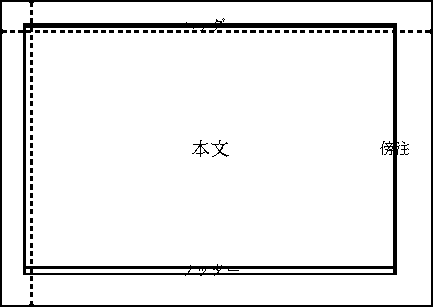
\includegraphics[scale=1]{geolay/geo11-1-crop.pdf}}%

%  vmargin=25mm,hmargin=15mm,
%  tmargin=25mm,bmargin=25mm,lmargin=15mm,rmargin=15mm,
%  top=25mm,bottom=25mm,left=15mm,right=15mm,

次は用紙サイズを A4 として,2段組,左右余白をそれぞれ 15\,mm,
上下余白を 25\,mm,段間の幅を 6\,mm,傍注・ヘッダー・フッター
なしの設定にします.

\GEO[\includegraphics]{a4paper,twocolumn,ignoreall,nomarginpar,noheadfoot,margin=\lb15mm\GQ25mm\rb,columnsep=6mm}{geolay/geo12-1-crop.pdf}{.3}{.7}
%\hbox{[scale=1]{geolay/geo12-1-crop.pdf}}%


%\endinput


\subsection{ヘッダやフッタの設定その1}\indindz{番号}{ページ}%
ヘッダやフッタなどに出力されるページ番号などを\zindind{ページ}{の番号}
変更したいときがあると思います.
\begin{Syntax}
\C{pagestyle}\pa{表示形式}
\end{Syntax}

\C{pagestyle}命令を記述したページから指定した\Z{表示形式}に変更されま
す.指定できる形式は\tabref{pagestyle}の通りです.


\begin{table}[htbp]
\begin{center}
\caption{ヘッダやフッタの指定}\tablab{pagestyle}
\begin{tabular}{ll}
\TR
\Th{命令}        & \Th{内容} \\
\MR
\str{empty}      & ページ番号を表示しない                \\
\str{plain}      & フッタ中央部に表示する              \\
\str{headings}   & ヘッダにページ番号と章・節名を表示する\\
\str{myheadings} & ユーザ定義の表示形式にする          \\
\BR
\end{tabular}
\end{center}
\end{table}

\qu{\str{myheadings}}では二つの命令によってヘッダの出力を指定します.

\begin{Syntax}
\Cmd{markright} \pa{ヘッダ} \\
\Cmd{markboth} \pa{偶数ヘッダ}\pa{奇数ヘッダ}
\end{Syntax}


片面印刷のときに \cmd{markright}を使います.
両面印刷には \Cmd{markboth}を使います.
2006年度版の\yo{○○△△大学}の論文集を
作成しているのであれば,例えば次のようにします.

\begin{InTeX}
\pagestyle{myheadings}
\markboth{○○△△大学論文集}{2006年度版}
\end{InTeX}


任意の1ページだけのヘッダ・フッタは,
次のようにする事でそのページだけ変えられます.

\begin{Syntax}
\Cmd{thispagestyle}\pa{表示形式}
\end{Syntax}


ページ番号の表示形式を変更するには \C{pagenumbering}命令を使います.

\begin{Syntax}
\Cmd{pagenumbering}\pa{表示形式}
\end{Syntax}

その場所から指定した形式で1ページ目からカウントしてページ番号を表示しま
す.指定できる表示形式は\tabref{pagenumber}の通りです.

\begin{table}[htbp]
\begin{center}
\caption{ページ番号の種類の指定}\tablab{pagenumber}
\begin{tabular}{lll}
\TR
\Th{形式}          & \Th{内容}          & \Th{出力例}         \\
\MR
\verb+arabic+ & \Z{アラビア数字}       & 1, 2, 3,\,\ldots \\
\verb+roan+   & \Z{ローマ数字}   & i, ii, iii,\,\ldots\\
\verb+Roman+  & ローマ数字   & I, II, III,\,\ldots\\
\verb+alph+   & アルファベット小文字& a, b, c,\,\ldots,\, z\\
\verb+Alph+   & アルファベット大文字& A, B, C,\,\ldots,\, Z\\
\BR
\end{tabular}
\end{center}
\end{table}
ここで注意する事はアルファベットにした場合は,
最大26ページまでしかカウントできないという事
です.27以上になった場合の対策は別にする事に
なります.

%もっと詳細なヘッダ・フッタ定義するときは自分で
%\cmd{ps@なんとか}というコマンドを定義してこれを
%\begin{InTeX}
%pagestyle{なんとか} 
%\end{InTeX}
%のように使います.本書で使われているスタイルは
%以下の通りです.\hito{奥村}{晴彦}の\cls{jsclasses}
%を少し変更しただけです.
%\begin{InTeX}
%\newcommand{\ps@myhead}{%
%  \let\@oddfoot\@empty
%  \let\@evenfoot\@empty
%  \def\@evenhead{%
%    \if@mparswitch \hss \fi
%    \underline{\hbox to \fullwidth{\autoxspacing
%        \textbf{\thepage}\hskip3zw\leftmark\hfill\@title}}%
%    \if@mparswitch\else \hss \fi}%
%  \def\@oddhead{\underline{\hbox to \fullwidth{\autoxspacing
%        \@title\hfill{\if@twoside\rightmark\else\leftmark\fi}%
%	\hskip3zw\textbf{\thepage}}}\hss}%
%  \let\@mkboth\markboth
%  \def\chaptermark##1{\markboth{%
%    \ifnum \c@secnumdepth >\m@ne
%      \if@mainmatter
%        \@chapapp\thechapter\@chappos\hskip1zw
%      \fi
%    \fi
%    ##1}{}}%
%  \def\sectionmark##1{\markright{%
%    \ifnum \c@secnumdepth >\z@ \thesection \hskip1zw\fi
%    ##1}}}%
%\end{InTeX}
%これを別ファイル\fl{hoge.sty}などにまとめて\cmd{usepackage}
%するか,\cmd{makeatletter}と\cmd{makeatother}で囲むかで
%実際の出力を確認してみてください.


\subsection{ヘッダ・フッタの変更その2\zdash\Y{fancyhdr}}
\indindz{スタイル}{ページ}%
\zindind{ページ}{スタイル}%
{\LaTeX}が標準で用意してくれているページスタイル
では寂しい,そう思う人も多いでしょう.自分で全て
定義する事もできますが,\Person{Piet}{Oostrum}が
作成した \Y{fancyhdr} を使うと比較的簡単にペー
ジスタイルをカスタマイズできます.\sty{fancyhdr}
は\Sty{fancyheadings}の後継で,ページのヘッダーと
フッターをカスタマイズできるマクロです.
まず\sty{fancyhdr}を使うために以下をプリアンブルに記述します.

\begin{InTeX}
\usepackage{fancyhdr} 
\pagestyle{fancy}
\end{InTeX}

\sty{fancyhdr}では
ヘッダ・フッタを六つに分割しています.
\begin{center}
\begin{tabularx}{\linewidth}{|XcX|}
\hline
\cmd{lhead} & \cmd{chead} & \hfill\cmd{rhead}\\
\multicolumn{3}{|c|}{%
   \hrulefill \pp{\cmd{headrulewidth}}\hrulefill} \\   
\multicolumn{3}{|c|}{\va{本文領域}}\\
\multicolumn{3}{|c|}{%
   \hrulefill \pp{\cmd{footrulewidth}}\hrulefill} \\
\cmd{lfoot} & \cmd{cfoot} &\hfill\cmd{rfoot} \\
\hline
\end{tabularx}
\end{center}
\Cmd{lhead},\Cmd{chead},\Cmd{rhead}の
三つはヘッダに使い\Cmd{lfoot},\Cmd{cfoot},
\Cmd{rfoot}の三つはフッタに使います.%
\indindz{罫線}{ヘッダ上部の}\indindz{罫線}{フッタ上部の}%%
\Cmd{headrulewidth}はヘッダ下部の罫線の太さで,
\Cmd{footrulewidth}はフッタ上部の罫線の太さです.
図だけのページや表だけのページはシンプルな
ヘッダ・フッタにしたり,ヘッダ下部の罫線を
引かない場合があります.その場合は \C{headrulewidth} を
\C{iffloatpage}命令で判定するように定義すると良いでしょう.

\begin{InTeX}
\def\headrulewidth{\iffloatpage{0pt}{.4pt}} 
\end{InTeX}

\cmd{lhead}などの
他の命令も同様に変更できます.

例えば\cls{jarticle}クラスで次のようなヘッダ・フッタ
\begin{center}
\begin{tabularx}{\linewidth}{|cXcXc|}
\hline
& & \hskip5em & \hfill 資本主義社会の崩壊 & \\
\cline{2-4}
\multicolumn{5}{|c|}{\va{本文領域}}\\
\cline{2-4}
& 名無しの権兵衛 & \hskip3em & \hfill \textbf{ページ番号} & \\
\hline
\end{tabularx}
\end{center}
を設定したければ以下のように記述します.

\begin{InTeX}
\lhead{} \chead{}
\rhead{資本主義社会の崩壊}
\lfoot{名無しの権兵衛} 
\cfoot{}
\rfoot{\textbf{\thepage}}
\def\headrulewidth{.4pt}
\def\footrulewidth{.4pt}
\end{InTeX}

書籍用クラス\cls{jbook}などでクラスオプションに
\Option{twoside}が指定されている場合は偶数ページと
奇数ページを個々に設定します.例えば次のような
ヘッダ・フッタにしたいとします.
\begin{center}
\begin{tabular}{|p{7zw}cp{7zw}|}
\hline
第1章\hskip1zw 序論& & \hfill 1.1\hskip1zw 背景\\\hline
\multicolumn{3}{|c|}{本文}\\\hline
& \textbf{2}&\hfill \\\hline
\end{tabular} \hfill
\begin{tabular}{|p{7zw}cp{7zw}|}
\hline
1.2\hskip1zw  目標& & \hfill 第1章\hskip1zw 序論\\\hline
\multicolumn{3}{|c|}{本文}\\\hline
& \textbf{3}& \\\hline
\end{tabular}
\end{center}
ヘッダ・フッタの奇数ページと偶数ページの場所
を区別するために以下のような設定になっています.
\begin{center}
\begin{tabular}{|p{6zw}cp{6zw}|}
\hline
\str{EL(H)}& \str{EC(H)}& \hfill  \str{ER(H)}\\\hline
\multicolumn{3}{|c|}{本文}\\\hline
\str{EL(F)}& \str{EC(F)} &\hfill \str{ER(F)} \\\hline
\multicolumn{3}{c}{偶数ページ側}\\
\end{tabular} \hfill
\begin{tabular}{|p{6zw}cp{6zw}|}
\hline
\str{OL(H)} &\str{OC(H)} & \hfill \str{OR(H)} \\\hline
\multicolumn{3}{|c|}{本文}\\\hline
\str{OL(F)}&\str{OC(F)} & \hfill  \str{OR(F)}\\\hline
\multicolumn{3}{c}{奇数ページ側}\\
\end{tabular}
\end{center}
先程の出力を得るためには \Cmd{fancyhead} と \Cmd{fancyfoot}命令を使います.

\begin{InTeX}
\documentclass{jbook}
\usepackage{fancyhdr} \pagestyle{fancy}
\fancyhead[ER,OL]{\rightmark}
\fancyhead[EL,OR]{\leftmark}
\fancyfoot[EC,OC]{\textbf{\thepage}}
\end{InTeX}

欧文のクラスではこれで良いのですが和文では \Cmd{chaptermark} と 
\Cmd{sectionmark}の定義を\sty{fancyhdr}を読み込んだ後に次のように定義
するのが普通でしょう.

\begin{InTeX}
 \def\chaptermark#1{\markboth{%
   \ifnum \c@secnumdepth >\m@ne
     \if@mainmatter
       \@chapapp\thechapter\@chappos\hskip1zw
     \fi
   \fi
   #1}{}}%
  \def\sectionmark#1{\markright{%
    \ifnum \c@secnumdepth >\z@ \thesection \hskip1zw\fi
    #1}}%
\end{InTeX}


\subsection{ページ/総ページ}

ヘッダ・フッタの設定をフッタだけに\yo{ページ/総ページ}にしたい場合がある
でしょう.これは例えば次のようにプリアンブルに記述します.

\C*{AtEndDocument}%
\C*{ps@total}%
\C*{@mkboth}%
\C*{@gobbletwo}%
\C*{@oddhead}%
\C*{@empty}%
\C*{@evenhead}%
\C*{@evenhead}%
\C*{@oddfoot}%
\C*{normalfont}%
\C*{thepage}%
\C*{hfil}%
\C*{@evenfoot}%
\begin{InTeX}
\AtEndDocument{\label{lastpage}}
\makeatletter
 \newcommand{\ps@total}{%
 \let\@mkboth\@gobbletwo
 \let\@oddhead\@empty
 \let\@evenhead\@empty
 \def\@oddfoot{\normalfont\hfil--\thepage/\pageref{lastpage}--\hfil}%
 \let\@evenfoot\@oddfoot}
\makeatother
\pagestyle{total}
\end{InTeX}

この場合は \cmd{ps@total}によって新規に\qu{\str{total}}という
ページスタイルを定義しています.ページ番号の書体を
変えたいときは \cmd{normalfont}を \cmd{bfseries}などに
変更します.


% hoge hoge

\section{レイアウトの制御}\indindz{ページ}{改}\indindz{区切り}{ページの}%
{\LaTeX}ではユーザが意図的に改行や改ページ
を行わなくても良いように工夫されています.ど
うしても自分の思い通りにページをレイアウト
できないときは強制的なレイアウト命令を使いま
す.{\K{ページ区切り}}を制御したいならば
\zindind{ページ}{の区切り}
\begin{description}
\item[\Cmd{newpage}] 
   改ページします.\Z{2段組}の場合は次の段までの
  改ページになります.
\item[\Cmd{clearpage}]	
   未出力の浮動体を配置してから改ページします.
 2段組の場合は本当の次のページまで改ページされます. 
\item[\Cmd{cleardoublepage}] 
  次のページが奇数ページになるように改ページします.
  これを{\KY{奇数起こし}}とか{\KY{改丁}}
  と呼びます.
\item[\Cmd{samepage}] 
   指定した場所でできる限り改ページを抑制します.
\end{description}
の四つの命令が使えます.

%\Cmd{nopagebreak}\opa{数値}\pp{$0 \leq i \leq 4$}\\
%\Cmd{pagebreak}\opa{数値} \\
%\Cmd{linebreak}\opa{数値} \\
%\Cmd{nolinebreak}\opa{数値} 



\textbf{空白}を制御するには以下の四つの命令が使えます.
\begin{description}
\item[\Cmd{hspace}\pa{長さ}] 
  長さ分の横方向の空白を挿入します.
  行頭では有効ではありません.
\item[\Cmd{hspace*}\pa{長さ}]
  行頭でも横方向の空白を挿入します.
\item[\Cmd{vspace}\pa{長さ}]
  長さ分の縦方向の空白を挿入します.
  ページの先頭・末尾では有効ではありません.\zindind{ページ}{の先頭での空き}
\item[\Cmd{vspace*}\pa{長さ}] \zindind{ページ}{の末尾での空き}
  ページの先頭・末尾でも縦方向の空白を挿入します.
\end{description}
これらの空白制御の命令では単位付きの長さで指定します.
\begin{InOut}
\hspace{1cm}空白制御用のコマンドは
行頭では意図的に\vspace{1cm}アスタ
リスクを付けます.\par\hspace{1cm}
段落の途中に縦方向\hspace{1cm}の空
白を挿入すると,段が改行されてから
縦に空白が挿入されます.
\end{InOut}

% geho


\section{その他のコマンド}
{\LaTeX}で用意されているその他のコマンドを紹介します.

\subsection{日付}
{\LaTeX}のプログラムを実行した段階で,その原稿をタ
イプセットした日付を保存しています.\C{hour} と \C{minute}
は\sty{jclasses}/\sty{jsclasses}でのみ使えます.
\begin{Syntax}
\begin{tabular}{*6l}
\C{today}&\pp{\Z{日付}} & \C{month}&\pp{\Z{月}} & \C{hour}  &\pp{\Z{時}}\\
\C{year} &\pp{\Z{年}}   & \C{day}  &\pp{\Z{日}} & \C{minute}&\pp{\Z{分}}\\
\end{tabular}
\end{Syntax}

\index{西暦}%
\index{和暦}%
使用しているクラスファイルによって出力が違います.\cls{jarticle}において
は \C{西暦}や,\C{和暦}という命令を使って \cmd{today} の西暦表示と和暦表
示を変更できます.\hito{奥村}{晴彦}の
\cls{jsclasses}で標準は西暦になっており,アスキーの
\cls{jclasses}では和暦が標準です\pp{個人的には天皇
制の名残のような和暦を使うのは好ましくないと感じ
ていますし,ビジネス文書でわざわざ和暦を使っても
世界に置いてけぼりを食らうだけだと思っています,
個人的に}.欧文のクラスファイルではその言語の標準
的な表示方法で出力されます.\index{年月日}\index{日付!\zdash の表示}
\cmd{today} 以外は \C{number} 等のカウンタの値を表示するコマンドを
必要とします\footnote{\C{two@digits} 命令を用いると
`2006/04/15'のように,ゼロが補われるようになります.}.
\begin{InOut}
今日は\number\year 年\number\month
月\number\day 日です.略して\today.
\end{InOut}

\subsection{{\protect\LaTeX}のロゴ}
\begin{Syntax}
\begin{tabular}{*3{l@{\space}l}}
 \C{TeX}   & \pp{\TeX} &
 \C{LaTeX} & \pp{\LaTeX} &
 \C{LaTeXe}& \pp{\LaTeXe} 
\end{tabular}
\end{Syntax}
\hito{奥村}{晴彦}の\Cls{jsclasses}ではこれらに加えて
次のロゴが用意されています.
\begin{Syntax}
\begin{tabular}{*3{l@{\space}l}}
 \C{pTeX}    & \pp{\pTeX}   &
 \C{pLaTeX}  & \pp{\pLaTeX} &
 \C{pLaTeXe} & \pp{\pLaTeXe}
\end{tabular}
\end{Syntax}
\begin{InOut}
「実は僕も{\TeX}使っています.」\\
「え?{\LaTeX}じゃないんですか?」\\
「いやぁ,僕は{\TeX pert}だからさ.
 {\LaTeXe}も使ってませんよ.」\\
「ということは{\pTeX}は使うんですね?」
\end{InOut}


\section{単位・通貨の出力について}\seclab{unit}
文中でも数式中でも単位は基本的にはローマン体で
出力するのが普通ですので
\begin{InOut}
それは$y=30cm$だから合計300mmだ.
\end{InOut}
のような入力はおかしい訳です.この場合は
\begin{InOut}
それは$y=30\,\mathrm{cm}$だから
合計300\,mmだ.
\end{InOut}
としたほうが良いでしょう\footnote{場合によっては`$y=30\,[\mathrm{cm}]$'
とする事もあると思います.}.
このように単位は数式中でも使う
事があるかもしれませんので \Cmd{ensuremath}で
単位用の命令を作成します.例えば長さの単位である`mm'は
次のように定義します.

\begin{InTeX}
\newcommand{\mm}{\ensuremath{\,\mathrm{mm}}}
\end{InTeX}

ただし{\LaTeX}ですでに定義されている
短い命令は再定義しないほうが無難ですので,リットル \textit{l}などは
次のようにします.

\begin{InTeX}
\newcommand{\litter}{\,\ensuremath{\mathit{l}}}
\end{InTeX}

日本ではリットルをイタリック体にする事もあるようですが,
基本的に単位は全てローマン体にしても良いようです.分野によっても
区別が違うので調べてください.毎回単位を定義するのも大変なので
単位用のマクロ\fl{units.sty}を以下のように作成します.

\begin{InTeX}
%File:units.sty
\newcommand{\mm}{\ensuremath{\,\mathrm{\milli mm}}}
\newcommand{\cm}{\ensuremath{\,\mathrm{cm}}}
\newcommand{\Km}{\ensuremath{\,\mathrm{Km}}}
\newcommand{\mg}{\ensuremath{\,\mathrm{mg}}}
\newcommand{\Kg}{\ensuremath{\,\mathrm{Kg}}}
\newcommand{\cc}{\ensuremath{\,\mathrm{cc}}}
\newcommand{\litter}{\,\ensuremath{l}}
\newcommand{\Ohm}{\ensuremath{\,\mathrm{\Omega}}}
\end{InTeX}

\yo{あの単位の命令はなんだったかなぁ}と考えてい
るよりも \cmd{mathrm}などを使ったほうが早いかもし
れません.

\begin{Prob}
\fl{units.sty}はかなり汎用性に欠ける書き方です.これを
どのような単位でも対応できるように一般化してください.

例えば`\cmd{U}'という単位を意味する命令を新規に定義するというならば,
おおむね次のようになります.

\begin{InTeX}
\newcommand*\U[1]{\ensuremath{\,\mathrm{#1}}}
\newcommand*\BU[1]{\ensuremath{\,[\mathrm{#1}]}}
\end{InTeX}

さらに `$x = 1\,[\mathrm{cm}]$'という出力を`\verb|$x = 1\BU{cm}$|'
として括弧付きで用いるようにするのも便利でしょう.
\end{Prob}

通貨などを出力するためには{\LaTeX}に標準で含まれる\Sty{textcomp}パッケー
ジを使うと良いでしょう.これは古いエンコーディングだと使えませんので
\Sty{fontenc}パッケージを読み込み次のようにします.

\begin{InTeX}
\usepackage[T1]{fontenc}
\usepackage{textcomp}
\end{InTeX}

フォントがビットマップになるという
事も危惧されますので特に不都合がなければ
\Sty{txfonts}や\Sty{pxfonts}を併用して

\begin{InTeX}
\usepackage{txfonts,textcomp}%とかpxfonts
\end{InTeX}

とするのがベターだと思います.\tabref{textcomp}が
\sty{textcomp}によって使用できる記号一覧です.\indindz{記号}{通貨}%%"
\begin{table}[htbp]\index{著作権記号}
\begin{scenter}
 \caption{\textsf{textcomp}で使える記号}\tablab{textcomp}
\begin{tabular}{L}
 \T{texttwelveudash}\\
 \T{textleftarrow}\\
 \T{textrightarrow}\\
 \T{textblank}\\
 \T{textdollar}\\
 \T{textquotesingle}\\
 \T{textdblhyphen}\\
 \T{textzerooldstyle}\\
 \T{textoneoldstyle}\\
 \T{texttwooldstyle}\\
 \T{textthreeoldstyle}\\
 \T{textfouroldstyle}\\
 \T{textfiveoldstyle}\\
 \T{textsixoldstyle}\\
 \T{textsevenoldstyle}\\
 \T{texteightoldstyle}\\
 \T{textnineoldstyle}\\
 \T{textlangle}\\
 \T{textminus}\\
 \T{textrangle}\\
 \T{textmho}\\
 \T{textbigcircle}\\
 \T{textohm}\\
 \T{textlbrackdbl}\\
 \T{textrbrackdbl}\\
 \T{textuparrow}\\
 \T{textdownarrow}\\
 \T{textasciigrave}\\
 \T{textborn}\\
 \T{textdivorced}\\
 \T{textdied}\\
 \T{textleaf}\\
 \T{textmarried}\\
 \T{textmusicalnote}\\
\end{tabular}
\begin{tabular}{L}
 \T{texttildelow}\\
 \T{textdblhyphenchar}\\
 \T{textasciibreve}\\
 \T{textasciicaron}\\
 \T{textgravedbl}\\
 \T{textacutedbl}\\
 \T{textdagger}\\
 \T{textdaggerdbl}\\
 \T{textbardbl}\\
 \T{textperthousand}\\
 \T{textbullet}\\
 \T{textcelsius}\\
 \T{textdollaroldstyle}\\
 \T{textcentoldstyle}\\
 \T{textflorin}\\
 \T{textcolonmonetary}\\
 \T{textwon}\\
 \T{textnaira}\\
 \T{textguarani}\\
 \T{textpeso}\\
 \T{textlira}\\
 \T{textrecipe}\\
 \T{textinterrobang}\\
 \T{textinterrobangdown}\\
 \T{textdong}\\
 \T{texttrademark}\\
 \T{textpilcrow}\\
 \T{textbaht}\\
 \T{textnumero}\\
 \T{textdiscount}\\
 \T{textestimated}\\
 \T{textopenbullet}\\
 \T{textservicemark}\\
 \T{textlquill}\\
\end{tabular}
\begin{tabular}{L}
 \T{textrquill}\\
 \T{textcent}\\
 \T{textsterling}\\
 \T{textcurrency}\\
 \T{textyen}\\
 \T{textbrokenbar}\\
 \T{textsection}\\
 \T{textasciidieresis}\\
 \T{textcopyright}\\
 \T{textordfeminine}\\
 \T{textcopyleft}\\
 \T{textlnot}\\
 \T{textcircledP}\\
 \T{textregistered}\\
 \T{textasciimacron}\\
 \T{textdegree}\\
 \T{textpm}\\
 \T{texttwosuperior}\\
 \T{textthreesuperior}\\
 \T{textasciiacute}\\
 \T{textmu}\\
 \T{textparagraph}\\
 \T{textperiodcentered}\\
 \T{textreferencemark}\\
 \T{textonesuperior}\\
 \T{textordmasculine}\\
 \T{textsurd}\\
 \T{textonequarter}\\
 \T{textonehalf}\\
 \T{textthreequarters}\\
 \T{texteuro}\\
 \T{texttimes}\\
 \T{textdiv}\\ 
\end{tabular}\\
\begin{tabular}{LC}
 \T{textpertenthousand} & 
 \T{textquotestraightbase}\\
 \T{textquotestraightdblbase} & 
 \T{textasteriskcentered}\\
 \T{textthreequartersemdash} & 
 \T{textfractionsolidus}\\
\end{tabular}

\end{scenter}
\end{table}
%
%tectcomp
%\T{textcapitalcompwordmark}
%\T{textascendercompwordmark}
%\T{textquotestraightbase}
%\T{textquotestraightdblbase}
%\T{texttwelveudash}
%\T{textthreequartersemdash}
%\T{textleftarrow}
%\T{textrightarrow}
%\T{textblank}
%\T{textdollar}
%\T{textquotesingle}
%\T{textasteriskcentered}
%\T{textdblhyphen}
%\T{textfractionsolidus}
%\T{textzerooldstyle}
%\T{textoneoldstyle}
%\T{texttwooldstyle}
%\T{textthreeoldstyle}
%\T{textfouroldstyle}
%\T{textfiveoldstyle}
%\T{textsixoldstyle}
%\T{textsevenoldstyle}
%\T{texteightoldstyle}
%\T{textnineoldstyle}
%\T{textlangle}
%\T{textminus}
%\T{textrangle}
%\T{textmho}
%\T{textbigcircle}
%\T{textohm}
%\T{textlbrackdbl}
%\T{textrbrackdbl}
%\T{textuparrow}
%\T{textdownarrow}
%\T{textasciigrave}
%\T{textborn}
%\T{textdivorced}
%\T{textdied}
%\T{textleaf}
%\T{textmarried}
%\T{textmusicalnote}
%\T{texttildelow}
%\T{textdblhyphenchar}
%\T{textasciibreve}
%\T{textasciicaron}
%\T{textgravedbl}
%\T{textacutedbl}
%\T{textdagger}
%\T{textdaggerdbl}
%\T{textbardbl}
%\T{textperthousand}
%\T{textbullet}
%\T{textcelsius}
%\T{textdollaroldstyle}
%\T{textcentoldstyle}
%\T{textflorin}
%\T{textcolonmonetary}
%\T{textwon}
%\T{textnaira}
%\T{textguarani}
%\T{textpeso}
%\T{textlira}
%\T{textrecipe}
%\T{textinterrobang}
%\T{textinterrobangdown}
%\T{textdong}
%\T{texttrademark}
%\T{textpertenthousand}
%\T{textpilcrow}
%\T{textbaht}
%\T{textnumero}
%\T{textdiscount}
%\T{textestimated}
%\T{textopenbullet}
%\T{textservicemark}
%\T{textlquill}
%\T{textrquill}
%\T{textcent}
%\T{textsterling}
%\T{textcurrency}
%\T{textyen}
%\T{textbrokenbar}
%\T{textsection}
%\T{textasciidieresis}
%\T{textcopyright}
%\T{textordfeminine}
%\T{textcopyleft}
%\T{textlnot}
%\T{textcircledP}
%\T{textregistered}
%\T{textasciimacron}
%\T{textdegree}
%\T{textpm}
%\T{texttwosuperior}
%\T{textthreesuperior}
%\T{textasciiacute}
%\T{textmu}
%\T{textparagraph}
%\T{textperiodcentered}
%\T{textreferencemark}
%\T{textonesuperior}
%\T{textordmasculine}
%\T{textsurd}
%\T{textonequarter}
%\T{textonehalf}
%\T{textthreequarters}
%\T{texteuro}
%\T{texttimes}
%\T{textdiv}
\sty{tectcomp}にも含まれていない通貨などを
探しているときはCTANに\Z{記号}の見本%
\footnote{\CTAN{info/symbols/comprehensive/}}が
ありますのでそちらを参照してください.

\section{あらかじめ定義されている見出しの変更}
\zindind{目次}{の見出しの変更}\zindind{見出し}{の変更}%
\yo{目次}や\yo{参考文献}などの見出しは \Cmd{tableofcontents}命令や
\Env{thebibliography}環境によって出力されます.
この見出しの文字を変更するには次のようにします.

\begin{InTeX}
\renewcommand{\refname}{関連書籍}
\end{InTeX}

標準的な和文の文書クラスでは\tabref{midas:henko}
の見出しが定義されています.

\begin{table}[htbp]
\begin{center}\zindind{図}{目次}\zindind{表}{目次}%
\indindz{目次}{図}%
\indindz{目次}{表}%
\zindind{部}{の見出し}%
\zindind{章}{の見出し}%
\zindind{目次}{の見出し}%
\zindind{参考文献}{の見出し}%
\zindind{索引}{の見出し}%
\zindind{付録}{の見出し}%
\zindind{図}{の見出し}%
\zindind{表}{の見出し}%
\caption{定義済みの見出しの変更}\tablab{midas:henko}
 \begin{tabular}{lll}
 \TR
 \Th{命令}            & \Th{意味} & \Th{標準的な定義}\\
 \MR
% \Cmd{prepartname}    & 部見出し番号の前の文字 & {第}\\
% \Cmd{postpartname}   & 部見出し番号の後の文字 & {部}\\
% \Cmd{prechaptername} & 章見出し番号の前の文字 & {第}\\
% \Cmd{postchaptername}& 章見出し番号の前の文字 & {章}\\
% \Cmd{contentsname}   & 目次の見出しの     & {目次}\\
% \Cmd{listfigurename} & 図目次の見出し   & \Z{図目次}\\
% \Cmd{listtablename}  & 表目次の見出し   & \Z{表目次}\\
% \Cmd{bibname}        & \env{thebibliography}環境の見出し& {参考文献}\\
% \Cmd{indexname}      & \env{theindex}環境の見出し& {索引}\\
% \Cmd{figurename}     & 図見出し番号の前の文字& {図}\\
% \Cmd{tablename}      & 表見出し番号の前の文字& {表}\\
% \Cmd{appendixname}   & \env{appendix}環境での見出しの前の文字& {付録}\\
 \C{prepartname}    & 部見出し番号の前の文字 & \Z{第}\\
 \C{postpartname}   & 部見出し番号の後の文字 & \Z{部}\\
 \C{prechaptername} & 章見出し番号の前の文字 & \Z{第}\\
 \C{postchaptername}& 章見出し番号の前の文字 & \Z{章}\\
 \C{contentsname}   & 目次の見出しの     & \Z{目次}\\
 \C{listfigurename} & 図目次の見出し   & \Z{図目次}\\
 \C{listtablename}  & 表目次の見出し   & \Z{表目次}\\
 \C{bibname}        & \env{thebibliography}環境の見出し& \Z{参考文献}\\
 \C{figurename}     & 図見出し番号の前の文字& \Z{図}\\
 \C{tablename}      & 表見出し番号の前の文字& \Z{表}\\
 \C{appendixname}   & \env{appendix}環境での見出しの前の文字& \Z{付録}\\
 \BR
 \end{tabular}
 \end{center}
\end{table}
\cmd{bibname}命令は\cls{jreport}や\cls{jbook}などでの定義で
\cls{(j)article}では \Cmd{refname}となっています.
\hito{奥村}{晴彦}の\cls{jsclasses}では節見出し番号の前と後にも
文字列を表示できるようになっています.

\begin{InTeX}
\renewcommand{presectionname}{第}
\renewcommand{postsectionname}{節}
\end{InTeX}

上記のように \Cmd{presectionname}や \Cmd{postsectionname}を
\K{再定義します}.

\section{目次再び}
目次に出力される項目を制御したいときがあります.例え
ば見出し命令にアスタリスクをつけた場合\pp{\Cmd{chapter*} など}は
通し番号が付かずに目次にも出力されません.
これを目次にも書き出すには次のようにします.

\begin{InTeX}
\addcontentsline{toc}{chapter}{なんとか}
\end{InTeX}

\begin{Syntax}
\Cmd{addcontentsline}\pa{拡張子}\pa{種類}\pa{要素}\\
\Cmd{addtocontents}\pa{拡張子}\pa{要素}
\end{Syntax}
例えば文書クラスに\cls{jreport}を使っていた場合に
\yo{謝辞}のような章を出力するときは次のように
入力します.

\begin{InTeX}
\chapter*{謝辞}
ありがとう,本当にありがとう.
\end{InTeX}

しかしこれを目次にも追加するには \cmd{chapter*} の直後に記述します.

\begin{InTeX}
\chapter*{謝辞}\addcontentsline{toc}{chapter}{謝辞}
ありがとう,本当にありがとう.
\end{InTeX}

目次や図目次のある部分で改ページしたいときには
次のようにします.

\begin{InTeX}
\addtocontents{toc}{\newpage}
\addtocontents{lof}{\newpage}
\end{InTeX}


%\subsection{自作の箇条書き型の環境}
%箇条書きとはいくつかの段落を改行や余白などを含めた一連
%の項目のことです.{\LaTeX}ではすでにこの箇条書き型の環
%境が登場しています.主な環境として
%\begin{itemize}
%\item ラベル付きの\env{itemize}環境.
%\item 番号付きの\env{enumerate}環境.
%\item 説明ラベル付きの\env{description}環境.
%\item 項目を中央揃えさせる\env{center}環境.
%\end{itemize}
%などがあります.箇条書き型の環境では項目の始めにラベルを
%付けて字下げを挿入します.ラベルや字下げは必ずしも必要では
%ないので,中央揃えさせるだけの\env{center}環境にも使えます.
%既存の箇条書き型環境で満足できないときは\Env{list}環境や,
%少し制限のある\Env{trivlist}環境のパラメータの変更を行います.
%
%\subsection{list環境}
%\Env{list}環境は汎用性の高い箇条書き型環境です.
%
%\begin{Syntax}
%\verb|\begin{list}|\pa{標準のラベル}\pa{設定}\\
%\va{項目}\\
%\verb|\end{list}|
%\end{Syntax}
%\begin{figure}[htbp]
% \begin{center}
%  \begin{picture}(300,500)(0,0)
%
%  \drawline(0,500)(0,450)(300,450)(300,500)%前のテキスト
%  \put(150,450){\mbox{箇条書き前の文章}}
%  \drawline(0,0)(0,50)(300,50)(300,0)%後のテキスト
%
%  \drawline(20,400)(70,400)(70,385)(20,385)(20,400)%ラベル1
%  \LRArrow(20,380){50}[\BS labelwidth]
%  \put(45,397){\makebox(0,0)[t]{ラベル1}}
%  \drawline(20,200)(70,200)(70,185)(20,185)(20,200)%ラベル2
%  \put(45,197){\makebox(0,0)[t]{ラベル2}}
%
%   %第1段落
%   \LRArrow(80,383){15}[] 
%   \put(110,380){\makebox(0,0)[t]{\texttt{\BS itemindent}}}
%   \LRArrow(70,400){25}[]
%   \put(90,403){\makebox(0,0)[b]{\texttt{\BS labelsep}}}
%  \drawline(80,385)(95,385)(95,400)(300,400)(300,350)(80,350)(80,385)
%
%  \end{picture}
%  \caption{\texttt{list}環境で設定できる値}
% \end{center}
%\end{figure}
%\subsection{trivlist環境}
% 
%
%\section{箇条書き環境の自作}
%
%\begin{Syntax}
%\Cmd{list}\pa{ラベル}\pa{命令} \va{項目} \cmd{endlist}\\
%\Cmd{item}
%\end{Syntax}
%
%\begin{Syntax}
%\verb|\begin{trivlist}| \va{項目} \verb|\end{endlist}|
%\end{Syntax}
%
%\begin{figure}[htbp]
%\begin{center}
%\setlength{\unitlength}{.4pt}
%\begin{picture}(400,500)(0,0)
%\put(0,0){\circle*{1}}
%\end{picture}
%\caption{リスト環境の形式}\figlab{listenv}
%\end{center}
%\end{figure}
%
%\begin{Syntax}
%\Cmd{leftmargin} (0)\\
%\Cmd{labelwidth} (0) \\
%\Cmd{itemindent} (0) \\
%\Cmd{linewidth} (\cmd{hsize})
%\end{Syntax}
%
%\begin{Syntax}
%\Cmd{makelabel} \\
%\Cmd{usecounter}\pa{hoge}
%\Cmd{boxlabels} 
%\end{Syntax}
%
%垂直空白(スキップ)
%\begin{Syntax}
%\Cmd{topsep} (0)\\
%\Cmd{partopsep} (0)\\
%\Cmd{itemsep} (0)\\
%\Cmd{parsep} (\cmd{parskip})
%\end{Syntax}
%
%水平空白(寸法)
%\begin{Syntax}
%\Cmd{leftmargin} ()\\
%\Cmd{rightmargin} (0pt)\\
%\Cmd{listparindent} (0pt)\\
%\Cmd{itemindent} (0pt)
%\Cmd{labelwidth} (0)
%\Cmd{labelsep} (0)
%\end{Syntax}
%
%\begin{Syntax}
%\Cmd{leftmargini} 
%\Cmd{leftmarginii} 
%\Cmd{leftmarginiii} 
%\Cmd{leftmarginiv} 
%\Cmd{leftmarginv} 
%\Cmd{leftmarginvi} 
%\end{Syntax}
%
%\Cmd{itemize}と\Cmd{enumerate}
%カウンタ\str{enumi},\str{enumii},\str{enumiii},\str{enumiv},
%

\section{多段組}\index{多段組}
{\LaTeX}では通常1段組と2段組しか制御できません.%
\zindind{2段組}{のときの段間}\zindind{2段組}{の段間の罫線}%
\begin{Syntax}
\begin{tabular}{ll}
 \Cmd{onecolumn}           & \\
 \Cmd{twocolumn}\opa{要素} & \\
 \Cmd{columnsep}          & \pp{2段組のときの段間}\\
 \Cmd{columnseprule}      & \pp{2段組のときの段間に引く罫線の太さ}
\end{tabular}
\end{Syntax}
1段組みにするためには \cmd{onecolumn}を使い,2段組に
するには \cmd{twocolumn}を使います.\cmd{twocolumn}
は改ページをしてから2段組を作成しようとします.
そのため任意引数に何らかの要素を与えるとその要素を
ページ上部に1段組で出力します.

\begin{Exe}
次の入力例をタイプセットし,その出力結果を吟味して下さい.

\begin{InTeX}
\columnsep 2zw
\columnseprule .4pt
\twocolumn[{\large\LaTeXe はどうです?}]
ここからの文章が2段組になるでしょう.{\LaTeX}での
多段組の実現は難しいそうです.
\end{InTeX}

\end{Exe}

%\begin{OutText}
%{\large\LaTeXe はどうですか}\\[2em] 
%\hfil\parbox[t]{.4\linewidth}{ここからの文章が
%2段組になるでしょう.{\LaTeX}での段組の
%実現}%
%\hskip1zw\makebox[.4pt][t]{%
%  \rule[-1\baselineskip]{.4pt}{2\baselineskip}}\hskip1zw%
%\parbox[t]{.4\linewidth}{は難しいそうです.}\hfil
%\end{OutText}
2段組みにすると図表は用紙の文章幅 \Cmd{textwidth}で
はなく1段分の幅 \Cmd{columnwidth}で張り込む事に
なります.また以下の二つの環境が使えます.
\begin{Syntax}
\Env{table*} 環境 \\
\Env{figure*} 環境
\end{Syntax}
\env{table}環境や\env{figure}環境にアスタリスクを付けると
その環境を1段分の幅でページの下部か上部に配置
しようとします.

\Cmd{twocolumn}を使って2段組をすると最終ページの
段の高さが揃わないので,格好悪いでしょう.これは
\sty{multicol}パッケージで2段組にすると段が揃いますし,
\Sty{balance}パッケージを使っても可能です.


\subsection{3段組以上の多段組\zdash\Y{multicol}}\seclab{multicol}
\Person{Frank}{Mittelbach}の作成した\Sty{multicol}を
使うと最高で10段まで段組できます.自動的に
段の終わりの最終ページの文章の高さを揃えてくれます.
星を付けると段の下端を揃えないようにするので,通常は星無しで用いると良い
でしょう.
%ただし商用利用のためには作者の許諾と使用料が必要です.
\begin{Syntax}
\verb|\begin{multicols|\pa{段数}\\
\va{文章内容}\\
\verb|\end{multicols}| 
\end{Syntax}
\Env{multicols}環境の場合は改ページされずに同じ
ページに違う段組を混在できます.余り好ましくない
事なので多用しないほうが良いでしょう.
以下のような入力があるとします.

\begin{InTeX}
\begin{multicols}{4}
このパッケージでは10段組まで多段組できますが, 同ページに違う段数の要素
を組み込むのは余り好ましいことではないので,特別な理由がない限り使うべき
ではありません.このパッケージでは段の終わりの最終ページの文章を自動で揃
えるので,従来の組版の規則にも合っています.
\end{multicols} 
\end{InTeX}

そうすると,次のような出力を得ることができます.

\begin{multicols}{4}
このパッケージでは10段組まで多段組できますが, 
同ページに違う段数の要素を組み込むのは余り
好ましいことではないので,特別な理由がない限り
使うべきではありません.このパッケージでは段の
終わりの最終ページの文章を自動で揃えるので,従
来の組版の規則にも合っています.
\end{multicols} 

\LaTeXe の標準では \C{onecolumn} と \C{twocolumn} によって 1 段組みと 2
段組みを切替える事もできます.

%\begin{InTeX}
%\documentclass[twocolumn]{jsarticle}
%\end{InTeX}

これによって全体の段組みを指定する事もできます.しかし, \C{onecolumn} と \C{twocolumn}
の両方とも改ページが必須で,ページの途中で段を変更する事もできなければ,
2 段組みのときに段の終わりが揃わないなどの制約があります .
%(普通の組版規則では
%ページの途中で段を変更するようなことはないので,これはこれで良いのだが).
%これを解消するためには \Person{Frank}{Mittelbach}の作成した (\emph{\TeX
%book} の多段組みアルゴリズムをベースに) \Y{multicol} パッケージを用いる
%と良いでしょう.%ただし,商用使用には payment とか donate とか色々.
%\begin{Syntax}
%\C{begin}\verb|{multicols*}|\pa{段数}\opa{多段組みを行なう前のテキスト}\\
%\va{多段組みを行なう要素}\\
%\C{end}\verb|{multicols*}|
%\end{Syntax}

%例えば,次のようなファイルがあるとします.
\Y{multicol} パッケージの制約として \E{table} 環境や \E{figure} 環境
で図表を出力する事ができません.そのかわり \E{table*} 環境並びに
\E{figure*} 環境で段を打ち抜いて図表を出力する事ができます.
この場合はページの上端か下端に配置されるようになります.
余白等を手動で調整する手間を惜しまないならば,次の入力例のように
自前の \E{mytable} 環境や \E{myfigure} 環境を定義する事ができます.

\begin{InTeX}
\documentclass[a4j,10pt,papersize]{jsarticle}
\newcommand*\mypict{\setlength\unitlength{1pt}%
  \begin{picture}(40,40)%
    \put(20,20){\circle*{10}}%
    \put(20,20){\circle{20}}%
  \end{picture}}%
\usepackage{multicol}
\columnseprule=.4pt
\columnsep=2zw
\multicolsep=1zw
\makeatletter
\def\myfigure{\vbox\bgroup\centering\def\@captype{figure}}
\def\mytable{\vbox\bgroup\centering\def\@captype{table}}
\def\endmyfigure{\egroup}
\def\endmytable{\egroup}
\def\hoge{\@tempcnta=\z@ \@whilenum \@tempcnta<100\do{%
   ほげほげ\advance\@tempcnta\@ne}。}
\makeatother
\begin{document}
\hoge
\begin{multicols}{3}
\hoge
\begin{equation}
 f(x)  = ax +b
\end{equation}
\hoge
\begin{figure*}[tb]
\centering\mypict
\caption{普通の\texttt{figure}環境での図だよ}
\end{figure*}
\hoge
\begin{myfigure}
 \mypict
 \caption{\texttt{multicols}環境中の図だよ}
\end{myfigure}
\hoge
\begin{mytable}
\begin{small}
  \caption{\texttt{multicols}環境中の表だよ}
 \begin{tabular}{lll}
 \hline
 \LaTeX & \LaTeXe& \LaTeX\,3\\
 \hline
 \end{tabular}
\end{small}
\end{mytable}
\hoge
\end{multicols}
\hoge
\begin{multicols}{4}[\section{新聞記事とか色々あるけどねぇ,どうだろう。}]
\hoge
\end{multicols}
\hoge
\begin{multicols}{5}
\hoge\par \hoge
\end{multicols}
\hoge 
\begin{multicols}{7}
\hoge\par \hoge
\end{multicols}
\end{document}
\end{InTeX}

上記の入力例の出力例は\figref{multicol}となります.

\begin{figure}[htbp]
   \IOmargin
   \makebox[0pt][l]{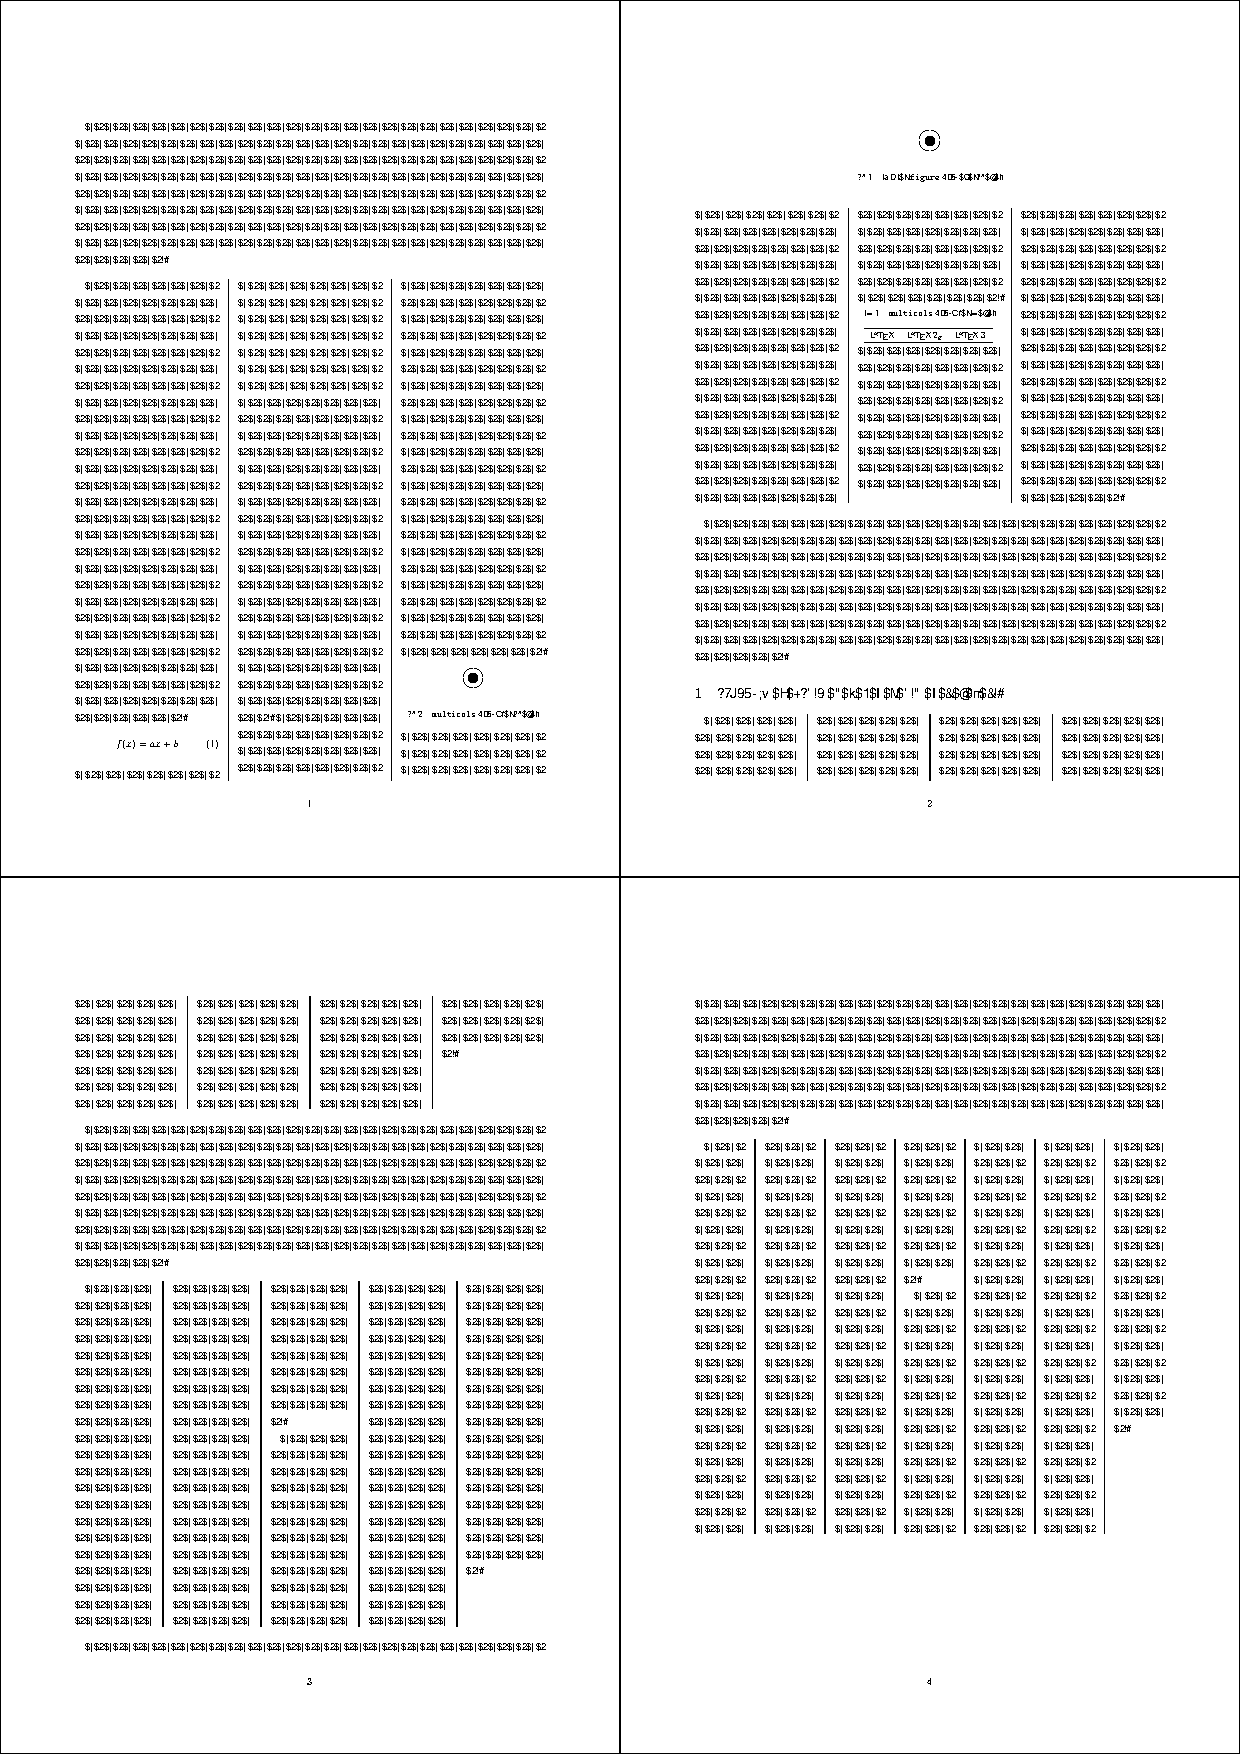
\includegraphics[width=\textwidth]{images/multicol.pdf}}
   \IOlabel
   \caption{\Y{multicol}の使用例の出力結果}\figlab{multicol}%
\end{figure}

\Person{Frank}{Mittelbach}の \Y{multicol} では 段抜きで配置する \E{figure*}
環境と \E{table*} 環境は許されますが,段の中に組まれる \E{figure}/\E{table}
環境は使えません.そのため,図をフロートさせずに配置するために
\E{myfigure}/\E{mytable} 環境を新設しています.ただし,フロートしない
ため図表の直前/直後で余計な空白が挿入されるので,これを手動で調整する (具
体的には関係する文の少し後に \E{myfigure}/\E{mytable} を記述する) 事に
なります.

段間の空白,段間に引かれる罫線,段の上端/下端の空きは次のように設定しま
す. 

\C*{columnseprule}%
\C*{columnsep}%
\C*{multicolsep}%
\begin{InTeX}
\columnseprule=.4pt % 段間に引かれる罫線
\columnsep=2zw %  段間の空白
\multicolsep=1zw % 段の上端/下端の空き
\end{InTeX}


\section{長さ} 
{\laTEX}における\K{長さ}には伸縮するものと
しないもの2種類があります.伸縮するものを
{\KY{可変長の長さ}}と呼び,伸縮しないものを\indindz{長さ}{可変長の}
{\KY{固定長の長さ}}と呼びます.\indindz{長さ}{固定長の}
可変長の長さは{\KY{スキップ}}と呼ばれる事が多いようですが,
本書では可変長の長さと呼びます.
可変長の長さは{\KY{長さ}},
{\KY{縮み率}},{\KY{伸び率}}の三つの
属性を持っています.固定長の長さは決まった値しか
持ちません.可変長の長さは縮み率と伸び率に従って
バネのように伸縮します.長さの定義には \cmd{newlength}が使えます.
\begin{Syntax}
\Cmd{newlength}\pa{綴り}\\
\Cmd{setlength}\pa{綴り}\pa{長さ} \\
\Cmd{addtolength}\pa{綴り}\pa{長さ}
\end{Syntax}
\cmd{setlength}で長さを設定します.\cmd{addtolength}
では元の長さにさらに長さを足します.\cmd{newlength}
で定義された長さは可変長にも固定長にもなって良い
事になっています.まず \cmd{newlength}で新規に
長さを定義します.次に \cmd{setlength}で
値を決めます.
\begin{InOut}
\newlength{\newa}\the\newa\\
\setlength{\newa}{10mm}\the\newa\\
\setlength{\newa}{10mm plus 3mm
   minus 2mm}\the\newa\\
\addtolength{\newa}{3mm}\the\newa
\end{InOut}
可変長の長さに値を足しても縮み率と伸び率には
影響しないのが例の出力から分かるでしょう.

長さを設定するには次の命令も使えます.
\begin{Syntax}
\Cmd{settowidth}\pa{綴り}\pa{要素} \\
\Cmd{settoheigth}\pa{綴り}\pa{要素} \\
\Cmd{settodepth}\pa{綴り}\pa{要素} 
\end{Syntax}
長さに対して要素の幅を代入するには \cmd{settowidth}を
使います.高さに関しては \cmd{settoheight},
深さには \cmd{settodepth}を使います.このような命令の
使い道を少し紹介しておきます.
\begin{InOut}
%\newlength{\newa} 
\newcommand{\fakewidth}[1]{%
  \settowidth{\newa}{#1}%
  \framebox[\the\newa][c]{\strut}}
解は{$\int f(x)dx$}となる.\par
解は\fakewidth{$\int f(x)dx$}となる.
\end{InOut}



\section{箱の操作}
まずは{\LaTeX}で用意されている{\KY{箱}}について説明します.
これらは\Fl{ltboxes.dtx}で定義されています.{\LaTeX}における箱とい
うのは文章や段落,数式や図表などの要素を格納する領域のようなものです.
{\LaTeX}の箱には\K{高さ}と\K{幅}と\K{深さ}の3種類の長さを
持っています.さらに箱のどの点を基準にするかという\K{基準点}と
いう座標も持ち合わせています.

\subsection{枠のない箱}
{\LaTeX}ではなんとも簡単に複数の要素を
一つの箱に収める事ができます.
\begin{Syntax}
\Cmd{makebox}\opa{幅}\opa{位置}\pa{要素}
\end{Syntax}

\cmd{makebox}では箱の幅と箱の中の要素の\indindz{幅}{箱の}%
位置を指定できます.箱の幅よりも要素の幅が狭いときに
箱の左側に配置\qu{\str l},中央に配置する\qu{\str c},
右側に配置する\qu{\str r},最後に要素を均一に配置する
\qu{\str s}の四つを使う事ができます.
\begin{InOut}
\makebox[3zw][l]{未来}と
\makebox[3zw][c]{函館}と
\makebox[5zw][r]{北海道}と
\makebox[5zw][s]{G o o d !}です.
\end{InOut}
要素の幅分の箱を作りたければ \cmd{mbox}を使います.
\begin{Syntax}
\Cmd{mbox}\pa{要素}
\end{Syntax}
引数を省略すると要素分の幅を確保し \cmd{makebox}を
使うよりも効率が良いです.
\begin{InOut}
\hspace*{\fill} 単なる予想ですが,
この箱の中では恐らく\mbox{改行が
起こりません.} 
\end{InOut}

\subsection{枠のある箱}


複数の要素を一つの塊として扱うようにするのが
{\LaTeX}における箱の役割のようなものです.
箱には枠を付ける事もできます.
\begin{Syntax}
\Cmd{framebox}\opa{幅}\opa{位置}\pa{要素}
\end{Syntax}
 \cmd{framebox}も \cmd{makebox}とほぼ同じですが\zindind{罫線}{の太さ}%
罫線の太さ \Cmd{fboxrule}と罫線と要素の
間隔 \Cmd{fboxsep}の二つの長さを設定できます.
 \cmd{fboxrule}は罫線の太さを, \cmd{fboxsep}は\zindind{枠}{の太さ}%
枠と要素との距離を長さで指定します.\zindind{枠}{と文字の間隔}%
\begin{InOut}
\framebox[3zw][l]{未来}と
{\fboxrule=3pt\framebox[3zw][c]{函
館}}と\framebox[5zw][r]{北海道}と
\framebox[5zw][s]{G o o d !}です.
\end{InOut}
 \cmd{makebox}と同じように引数を省略すると要素分の
幅を確保する \cmd{fbox}が使えます.
\begin{Syntax}
\Cmd{fbox}\pa{要素}
\end{Syntax}
\begin{InOut}
これは{\fboxsep=0pt\fbox{ぴったり
です}}.こちらは{\fboxrule=.8pt
\fbox{若干太い}}.
\end{InOut}

\subsection{広範囲な箱}\indindz{箱}{広範囲な}%

指定した箱の大きさで段落を組む \Cmd{parbox}
命令もあります.標準では字下げがされません\indindz{字下げ}{箱の中での}%
ので必要があれば \cmd{parindent}に長さを代入
してください.
\begin{Syntax}
\Cmd{parbox}\opa{位置}\opa{高さ}\opa{要素の位置}\pa{幅}%
\pa{文字列}
\end{Syntax}
\cmd{parbox}で作成された箱の基準をどこにするのかを
\va{位置}で指定します.位置には上部\qu{\str t},
中央\qu{\str c},下部\qu{\str b}の三つが使えます.
標準では中央になります.
\begin{InOut}
\parbox{13zw}{段落が終わる命令\par
を使っても改行されますが\par
標準では字下げされません.}
\end{InOut}
\begin{InOut}
\parbox[c]{4zw}{箱が中央に.}\ldots
\parbox[t][3zw][c]{4zw}{文字が中央,
上が基準}\ldots 
\parbox[b][3zw][t]{4zw}{文字が下に,
下が基準}\ldots
\end{InOut}
\zindind{ページ}{のような箱}ページのような箱を組む\env{minipage}環境もあります.
\begin{Syntax}
\verb|\begin{minipage}|\opa{位置}\pa{幅}\\
ページ内容\\
\verb|\end{minipage}|
\end{Syntax}
\Env{minipage}環境では段落が組まれますし,
脚注の出力も可能です.%
\index{脚注!minipage環境での@\texttt{minipage}環境での\zdash}%
\begin{InOut}
この環境は~
\begin{minipage}[t]{7zw}
ページを組みあげるので脚注%
\footnote{脚注です.}
もページの中に出力されます.
\end{minipage} 
~となります.
\end{InOut}

\subsection{箱の保存と使用}\zindind{箱}{の保存}\zindind{箱}{の再利用}%%
ある要素を箱の中に保存し,それを再利用できれば
エネルギー消費を減らす事ができます.
\begin{Syntax}
\Cmd{newsavebox}\pa{綴り}
\end{Syntax}
箱を保存するためには保存する場所の確保を \cmd{newsavebox}で
行います.{\LaTeX}が使っ
ても良い箱は数が限られているのであらかじめ
いくつくらい使うのかを宣言してあげます.
宣言するときはバックスラッシュを先頭に付けます.
箱の中に要素を保存するときは \cmd{savebox}か \cmd{sbox}命令を使います.
\begin{Syntax}
\Cmd{savebox}\pa{綴り}\opa{幅}\opa{要素の位置}\pa{要素}\\
\Cmd{sbox}\pa{綴り}\pa{要素}
\end{Syntax}
箱の幅や要素の位置を指定するときは \cmd{savebox}
を使います.もちろん幅を指定しないと要素の位置は
指定できません.
上記の命令のほかにも\Env{lrbox}環境があります.
行に収まるくらいの要素を\env{lrbox}環境の中に
記述すると\va{綴り}の箱に代入します.
\begin{Syntax}
\verb|\begin{lrbox}|\pa{綴り}\\
\va{要素}\\
\verb|\end{lrbox}|
\end{Syntax}

これまでの命令では箱を用意してその中に要素を保\zindind{箱}{の用意}%
存するだけですので,保存した箱を \Cmd{usebox}命令で使います.
\begin{Syntax}
\Cmd{usebox}\pa{綴り}
\end{Syntax}
\cmd{usebox}命令を使うと\va{綴り}の箱に
保存されている要素を複数回再利用できます.
\begin{InOut}
\newsavebox{\hoge} 
\savebox{\hoge}{\LaTeXe から
  \LaTeX\,3 へ}
\usebox{\hoge}, \usebox{\hoge}.\\
\usebox{\hoge}, \usebox{\hoge}.\\
\sbox{\hoge}{}  \usebox{\hoge}
\end{InOut}
{\LaTeX}の作業領域は限られていますので \Cmd{setbox}命令で\va{綴り}の箱を
使い終わったら空にします.


\subsection{箱の上げ下げ}\zindind{箱}{の上げ下げ}%
ある要素を箱の中に入れて,さらに上げ下げを
同時に行う \Cmd{raisebox}命令もあります.
\begin{Syntax}
\Cmd{raisebox}\pa{上げ下げ}\opa{高さ}\opa{深さ}\pa{要
 素}
\end{Syntax}
\cmd{raisebox}命令の中には文字列や他の箱も
挿入できます.
\begin{InOut}
それで,\raisebox{1zw}{あれ}は
\raisebox{-1zw}{これ}で,
\raisebox{1.5zw}{\fbox{枠付きの箱}}だ.
\end{InOut}


\subsection{罫線と下線}

箱とは違うのですが\KY{罫線}をここで紹介しておきます.
\begin{Syntax}
\Cmd{rule}\opa{上げ率}\pa{幅}\pa{高さ}
\end{Syntax}
 \cmd{rule}命令は使いものになります.見えない罫線を
引く事もできます.例えば幅が0\,ptでも高さのある
罫線,高さが0\,ptでも幅のある罫線が使えますから,
こんな使い方もできるわけです.枠の見える
状態での例を見てください.
\begin{InOut}
\newcommand*\RULE[2]{%
  \rule{0pt}{#1}\rule{#2}{0pt}}
未来 \fbox{\RULE{3zw}{4zw}}
函館 \fbox{\RULE{3zw}{2zw}}
\end{InOut}

箱とは違うのですが\KY{下線}も紹介しておきます.
下線は \cmd{underline}を使います.
\begin{Syntax}
\Cmd{underline}\pa{要素}
\end{Syntax}
 \cmd{underline}の中に箱を入れる事もできますし,
何を入れても構いません.
\begin{InOut}
\underline{\fbox{枠付きの箱}の下線}
はこのようにしますし,もちろん
\underline{下線}も表示できます.
\end{InOut}

\subsection{枠付きの箱その2\zdash\Y{fancybox}}\indindz{箱}{枠付きの}%
{\LaTeX}の標準では \Cmd{fbox}と \Cmd{framebox}命令が使えます.
\indindz{枠}{2重の}%
\begin{InOut}
\fbox{これは枠付きの箱} \\
\framebox[10zw][c]{日本太郎}\\
\fbox{\fbox{2重枠の箱}} \\
{\fboxrule=1pt\fbox{枠の太い箱}}\\
{\fboxsep=0pt\fbox{文字と枠がぴったり
な箱}}
\end{InOut}

\Person{Timothy}{Zandt}による\Sty{fancybox}を使ってみると
枠付きの箱を出しやすいでしょう.枠付きの箱に文字列を入れる
ための命令として \Cmd{shadowbox},\Cmd{doublebox},
\Cmd{ovalbox},\Cmd{Ovalbox}の四つがあります.
\begin{InOut}
\shadowbox{影付きの箱} \\
\doublebox{2重の枠 \\
\ovalbox{辺が丸い箱} \\
\Ovalbox{太くて辺が丸い箱}}
\end{InOut}

\sty{fancybox}を使うと\Env{Sbox}環境というものが使えて,
これは環境内のものを箱\pp{レジスタ}である \Cmd{TheSbox}に
保存します.このようにして保存した箱を \Cmd{fbox}などで
囲みます.例えば\env{minipage}を枠で囲む\env{fminipage}
環境を作成するのであれば次のようにします.

\begin{InTeX}
\newenvironment{fminipage}%
  {\begin{Sbox}\begin{minipage}}%
  {\end{minipage}\end{Sbox}\fbox{\TheSbox}}
\end{InTeX}


\begin{InOut}
\newenvironment{fminipage}%
  {\begin{Sbox}\begin{minipage}}%
  {\end{minipage}\end{Sbox}%
   \fbox{\TheSbox}}
\begin{fminipage}{.8\linewidth}
この環境は枠で囲まれます.というか,
囲んでくれないと困ります.
\end{fminipage}
\end{InOut}

数式環境などを枠で囲もうと思うとき,数式番号も
含めて枠の中に入れるのはちょっと面倒かもしれません.
\cmd{fbox}などの命令を使うとそこから数式を組み立てる
モードではなく文章を組み立てるモードになりますので,
もう1度数式環境を書きます.
\begin{InOut}
\( y = f(x) + \fbox{\(C\)}\) 
\begin{equation}
 \fbox{\(y = f(x)\)}
\end{equation}
\end{InOut}

番号付きの数式を文章幅いっぱいに枠で囲むには
\begin{quote}
 (\cmd{linewidth} \pp{文章幅} $-2$\cmd{fboxrule} $-2$\cmd{fboxsep})
\end{quote}
を計算します.これには\Sty{calc}パッケージが使えます.
\begin{InOut}
\usepackage{calc,fancybox} 
\fbox{\parbox{(\linewidth-
   2\fboxrule-2\fboxsep)}{
\begin{equation} y=f(x) 
\end{equation}}}
\end{InOut}

\env{eqnarray}環境は枠で囲もうと思うと\sty{fancybox}の
場合は\Env{Beqnarray}が用意されていますので,こちらの
環境を \cmd{fbox}などで囲みます.
\begin{InOut}
\fbox{\begin{Beqnarray}
 y & = & f(x)\\
   & = & 1/x
\end{Beqnarray}} 
\end{InOut}

\env{table}環境や\env{figure}環境などで見出しも
含まれる要素は \Cmd{Sbox} で一度保存したものを枠で
囲むようにします.こうすると
\begin{InTeX}
\usepackage{calc,fancybox}% プリアンブルで
\newenvironment{ftable}[1][htbp]%
  {\begin{table}[#1]
   \begin{Sbox}\begin{minipage}{%
  (\linewidth-2\fboxrule-2\fboxsep)}}%
  {\end{minipage}\end{Sbox}\fbox{\TheSbox}\end{table}} 
\end{InTeX}
のように\env{ftable}や\env{ffigure}のような環境が
定義できます.この出力例が\tabref{fancy}となります.
\begin{ftable}
\begin{center}
  \caption{\protect\LaTeX の歴史}\tablab{fancy}
  \begin{tabular}{ccc}
 \LaTeX\,2.09& \LaTeXe& \LaTeX\,3\\
 \end{tabular} 
\end{center}
\end{ftable}

\sty{fancybox}では\env{center}環境のように行揃えを
行う環境があります.これを枠で囲むには%
\zindind{左揃え}{を枠で囲む}%
\zindind{右揃え}{を枠で囲む}%
\zindind{中央揃え}{を枠で囲む}%
\Env{Bcenter},\Env{Bflushleft},\Env{Bflushright}
環境を使います.
\begin{InOut}
\fbox{\begin{Bcenter}
ここは \\ 中央揃えで \\ 
  枠付きです.
\end{Bcenter}}
\end{InOut}
\begin{InOut}
\fbox{\begin{Bflushleft}
ここは \\ 左揃えで \\ 
  枠付きです.
\end{Bflushleft}}
\end{InOut}
\begin{InOut}
\fbox{\begin{Bflushright}
ここは \\ 右揃えで \\ 
 枠付きになります.
\end{Bflushright}}   
\end{InOut}
\env{minipage}環境の中で行揃えの命令を使う事も
考えられますが,その場合は横幅を指定しないといけ
ないので,これらの環境は便利でしょう.
箇条書き環境も同様に\env{minipage}の中に入れて \cmd{fbox}で
囲む事も考えられますが,\sty{fancybox}では
\Env{Bitemize},\Env{Benumerate},\Env{Bdescription}の
三つがすでに定義されているので,これらの環境を
枠で囲みます.
\begin{InOut}
\fbox{\begin{Benumerate}
 \item 北海花子.
 \item 太郎君と花子さん.
 \item 日本太郎.
\end{Benumerate}}
\end{InOut}

\begin{comment}
 変換のときに
 ** WARNING ** Object reference with key "enumi.x.xx" is in use.
 ** WARNING ** Could not add Dests name tree entry...
 が出てくるかが,気にしないでね.
\end{comment}

\Cmd{verb}命令を枠で囲むときは \Cmd{VerbBox}命令を
使います.
\begin{InOut}
\VerbBox{\fbox}{
\verb|\VerbBox{\fbox}{\verb+\+}|}
\end{InOut}

\Env{verbatim}環境を枠で囲む場合はやはり先に
\env{Sbox}環境で囲んで \cmd{TheSbox}を枠で
囲むようにします.この場合\Env{fverbatim}環境を
定義したほうが便利でしょう.ただし,
この場合 \Cmd{VerbatimEnvironment}命令と\Env{Verbatim}環境を
併せて使わないとエラーになります.
\begin{InOut}
\newenvironment{fverbatim}[1]%
 {\VerbatimEnvironment 
 \begin{Sbox} \begin{minipage}{#1}%
 \begin{Verbatim}}{\end{Verbatim}%
  \end{minipage}\end{Sbox}%
  \fbox{\TheSbox}}
\begin{fverbatim}{.8\linewidth}
このべた書き環境は枠で囲まれて
出力されます.
\end{fverbatim}
\end{InOut}


枠付の箱を出力するために \LaTeX 標準の \E{framebox}環境
や \C{fbox} などが使用できますが,
もうすこし,角がまるかったり,数式などにも使えると便利です.
ある程度は好き好きシリーズの初級編で取り扱っているので,そちらを参照して
下さい.ここでは\Person{Timothy}{Zandt}による \Y{fancybox} をもう少し
細かく見てみましょう.
\begin{Syntax}
\C{boxput*}\xy{x}{y}\pa{下になる要素}\pa{上になる要素}
\end{Syntax}
という \C{boxput} 命令が使えます.使用例を参考にしてみて下さい.
\C{boxput} に星を付けると重ね合わせる順番が逆になります.
\begin{InOut}
\usepackage{fancybox,color}
\boxput(0,0){\color{blue}\Huge Draft}
{\color{red}\parbox{\linewidth}{%
こちらはなんでもかんでも\LaTeX 
でがんばります.\LaTeX は最高で
す.とにかく一度使ってみて下さい.}}
\end{InOut}
他にもページごと枠で囲む \C{fancyput} や \C{thisfancyput} なども
あります.
\begin{Syntax}
\C{fancyput*}\xy{x}{y}\pa{文章要素} \\
\C{thisfancyput*}\xy{x}{y}\pa{文章要素} 
\end{Syntax}
ここでは触れませんが \E{verbatim} 環境系の拡張がされています.


このほかにも\sty{fancybox}にはファイルから
読み込んだ行をべた書き環境に出力する命令なども
用意されています.





\section{空白の挿入}
{\LaTeX}にはいろいろ空白が用意されているのですが,
それらは{\KY{空き}}に含まれます.単語間に挿入される
程度の空きを基準とするとその4倍の空きを
\qu{quad}\pp{クワタ}と呼びます.和文組版では
空きの基準となるのは全角1文字分の幅であり,これを
\emph{全角空白}などと呼びます.全角空白一つ分の
空きを\emph{全角空き},全角空白二つ分の空きを
\emph{倍角空き}と呼びます.さらに4分の1の場合は
\emph{四分空き},6分の5ならば\emph{二分三分}と
呼んだりします.欧文の\qu{quad}と和文の\yo{クワタ}
では若干長さが異なりますので,本書では二つを
区別して表します.

\subsection{水平方向の空き}
\indindz{空き}{水平方向の}
\zindind{改行}{を許す空き}%
水平方向の空きにはその両側での改行を許すものと
許さないものがあります.主な空きを制御する
命令は\tabref{yokokuhaku:break}の通りです.
\tabref{yokokuhaku:break}は基本的に
空きの前後での改行を行っても良い事になっています.
\begin{table}[htbp]
\begin{center}
\caption{改行を許す水平方向の空き}\tablab{yokokuhaku:break}
\glossary{" @\hspace*{-1.2ex}\verb*+"\" +}%"
\indindz{空白}{単語間}%
\begin{tabular}{ll}
\TR
\Th{命令}         & \Th{意味}  \\
\MR
\verb*|\ |   & 適切な\emph{単語間空白} \pp{約1/4\,quad分}  \\
\C{quad}   & 1\,quad分の空き \\
\C{qquad}  & 2\,quad分の空き \\
\C{enspace}& 1/2\,quad分の空き\\
\C{enskip} & 適切な約1/2\,quad分の空き\\
\C{thinspace}    & 1/5\,quad分の空き\\
\C{negthinspace} & $-$1/5\,quad分の空き\\
\BR
\end{tabular}
\end{center}
\end{table}

%\tabref{yokokuhaku:break}は基本的に
%空きの前後での改行を行っても良い事になっています.

\begin{InOut}
ユーザが{\quad}原稿の中{\qquad}で空き
の調節を直接\ するのは好ましくない.
\end{InOut}

\tabref{yokokuhaku:break}の命令は改行を
許しますが\tabref{yokokuhaku:nobreak}では
空きの前後での改行を許しません.
\zindind{改行}{を許さない空き}%
改行を許さないので行頭・行末が不揃いに\index{行末}
なるときがあります.


\begin{table}[htbp]
\begin{center}
\caption{改行を許さない水平方向の空き}\tablab{yokokuhaku:nobreak}
\glossary{" @\hspace*{-1.2ex}\verb+"\"!+}%
\index{"~@\verb+"~+}%"
\glossary{"~@\verb+"~+}%"
\begin{tabular}{ll}
\TR
\Th{命令}     & \Th{意味}  \\
\MR
\Cmd{,}  & 3/18\,quad分の空き\\
\Cmd{:}  & 4/18\,quad分の空き\\
\Cmd{;}  & 5/18\,quad分の空き\\
\verb|\!|& $-3/18$\,quad分の空き\\
\verb|~| & 適切な\emph{単語間空白} \\
%\Cmd{hspace*}\pa{長さ}& 
\BR
\end{tabular}
\end{center}
\end{table}

%改行を許さないので行頭・行末が不揃いに\index{行末}
%なるときがあります.

\begin{InOut}
Donald~E. Knuth made \TeX\@. 
Leslie~Lamport made \LaTeX\@.
\end{InOut}

自分で水平方向の空きの長さを指定するならば \Cmd{hspace*}
命令が使えます.
\begin{Syntax}
\Cmd{hspace*}\opa{長さ}
\end{Syntax}
アスタリスクを付けると行頭・行末でも使えるようになります.
\begin{InOut}
日本太郎\hspace{2zw}ならば\par
\hspace*{-2zw}である.
\end{InOut}
\hito{奥村}{晴彦}の\Cls{jsclasses}を使っているときに
は\qu{\str{pt}}や\qu{\str{cm}}などの単位は使わずに
\qu{\str{truept}}や\qu{\str{truecm}}などを使わないと
長さがずれます.これが面倒ならば文章で使用されている
フォントに応じて基準の変わる\qu{\str{em}}や\qu{\str{zw}}
などを使ってください.

\subsection{垂直方向の空き}
\indindz{空き}{垂直方向の}

自分で長さを指定する垂直方向の空きにおいて
は \cmd{addvspace}と \cmd{vspace*} の二つが使えます.
\cmd{vspace*} はアスタリスクを付けないとページの最上部・最下部
では有効になりません.あらかじめ長さの決まっている
垂直方向の空きとして \cmd{smallskip},\cmd{midskip},
\cmd{bigskip}の三つがありますが,これは\emph{スキップ}
と呼ばれるもので可変長の空きが挿入されます.
%\yo{大体で良いからこれくらいの空きを入れてね.}程度の
%意味を持っています.
\yo{見映えが損なわれない程度におおよそ指定した長さの空きを挿入してほしい}と
いうような意味合いを持っています.
\begin{table}[htbp]
\begin{center}
\caption{垂直方向の空き}\tablab{tatekuhaku}
  \begin{tabular}{ll}
 \TR
 \Th{命令}            & \Th{意味} \\
 \MR
 \C{smallskip}& 3\,pt $\pm$1\,ptの空き \\
 \C{medskip}  & 6\,pt $\pm$2\,ptの空き \\
 \C{bigskip}  & 12\,pt \pp{$+$4\,ptか $-$2\,pt} の空き \\
 \BR
 \end{tabular}
\end{center}
\end{table}
垂直方向の空きは紙面の多くの部分を空きで占有するので
無駄が多くなります.{\LaTeX}では図表と段落のあいだや
そのほか必要と思われる所には半自動的に
空きが挿入されるようになっておりますので,闇雲に
垂直方向の空きを挿入するのは好ましくないと思われます.

長さを自分で指定して空きを挿入する場合
は \cmd{vspace*} と \cmd{addvspace}が使えます.
\begin{Syntax}
\Cmd{addvspace}\pa{長さ}\\
\Cmd{vspace*}\pa{長さ} 
\end{Syntax}
\cmd{vspace*} のアスタリスクを外すとページの最上部・最下部での
空きの挿入が有効になりません.\cmd{addvspace}は
直前の空きがどれくらいかも調べているので \cmd{vspace}
よりも適当な空きを挿入します.
\begin{InOut}
この\vspace*{2zw}だと全角2文字分の
垂直方向の空きが挿入されると思われます.
\end{InOut}


\section{伸縮する糊}
{\LaTeX}ではバネのように伸縮する\emph{糊}のような
便利な道具があります.これは活版印刷時代における
活字職人が経験で挿入する\KY{込め物}に似ています.

{\LaTeX}においてもある領域の中での空きを制御するためとか,適切な表示をす
るための込め物が使われます.{\LaTeX}で使われる込め物は{\KY{グルー}}と呼
ばれています.グルーは伸縮自在でバネのように要素と要素をくっ付けるので伸
縮する\emph{糊}とも呼ばれています.

グルーは特別な単位\qu{\str{fil}}と\index{fil@\texttt{fil}}%
\index{fill@\texttt{fill}}\qu{\str{fill}}によって定義されています.
\qu{\str{fil}}は良い\ruby{按}{あん}\ruby{排}{ばい}
で0からかなり大きい空きまで挿入する働きを
します.\qu{\str{fill}}は\qu{\str{fil}}よりも
大きく無限に近い空きを挿入する働きをします.
\begin{table}[htbp]
\begin{center}
\caption{{\protect\LaTeX}で使用できるグルー}
\tablab{gulue:fil}
  \begin{tabular}{ll}
 \TR
 \Th{命令}  & \Th{意味} \\
 \MR
 \Cmd{hfil}  & 水平方向にかなり大きく伸びる空き\\
 \Cmd{hfill} & 水平方向に無限に大きく伸びる空き\\
 \cmd{hss}   & 水平方向にかなり大きく伸び縮みする空き\\
 \MR
 \cmd{vfil}  & 垂直方向にかなり大きい空き\\
 \cmd{vfill} & 垂直方向に無限に大きい空き\\
 \cmd{vss}   & 垂直方向にかなり大きく伸び縮みする空き\\
 \BR
 \end{tabular}
\end{center}
\end{table}
\qu{\str{fil}}は\qu{\str{fill}}よりも弱いので
\qu{\str{fill}}のほうが優先されます.
\begin{InOut}
この空き{\hfil}は{\hfil}かき消されません.\par
この空きは{\hfil}恐らく{\hfill}かき消されます.
\end{InOut}
\qu{\str{fil}}と\qu{\str{fill}}の二つのグルーの
両方を使っている場合は空きが挿入されない場合があ
りますから気を付けてください.

もう少し相対的なグルーを挿入するには
\cmd{stretch}を使います.
\begin{Syntax}
\Cmd{stretch}\pa{整数}
\end{Syntax}
これは\qu{\str{fill}}の何倍かのグルーを挿入しても
良いようにするために使用できます.
\begin{InOut}
hoge\hspace{\stretch{3}}hoge%
\hspace{\stretch{1}}hoge.\par
hoge\hspace{\fill}hoge\hspace{\fill}
hoge.\par
\end{InOut}
\Cmd{fill}は \cmd{hspace}や \cmd{vspace}の引数に
使う事ができるグルーです.
例えばページの最上部に無限に近いグルーを
挿入するときは以下のようにします.
\begin{InOut}
\vspace*{\fill}を使ってもこの出力例で
は伸びません.
\end{InOut}

\subsection{空白ではないグルー}
\cmd{hfil}や \cmd{hfill}は空白を挿入するグルーでした.そうではなく,与え
られた領域を程よく文字列や要素で埋めてくれる込め物もあると便利です.目次
でも使われているのがお分かりになるでしょう.これらを{\KY{リーダ}}と呼び
ます.{\LaTeX}であらかじめ定義されているリーダは\tabref{leaders}となりま
す.

\qu{\str{fill}}ですから無限に伸びます.
\begin{table}[htbp]
\begin{center}
\caption{主なリーダ}\tablab{leaders}
\begin{tabular}{lp{10zw}}
\TR
\Th{命令} & \Th{出力例} \\
\MR
\Cmd{dotfill}	    & \dotfill\\
\Cmd{hrulefill}     & \hrulefill\\
\Cmd{leftarrowfill} & \leftarrowfill\\
\Cmd{rightarrowfill}& \rightarrowfill\\
\Cmd{downbracefill} & \downbracefill\\
\Cmd{upbracefill}   & \upbracefill\\
\BR
\end{tabular}
\end{center}
\end{table}
\cmd{dotfill}と \cmd{hrulefill}は\Fl{ltplain.dtx}で,
それ以外は\Fl{fontdef.dtx}にて定義されています.
段落中で使うと段の終わりまで伸びます.
\begin{InOut}
\makebox[5zw][l]{未\dotfill 来}\\
\hrulefill\\
北海\leftarrowfill 道と\\
北方領土\rightarrowfill\par
\end{InOut}
これらのリーダは \Cmd{leaders}という命令によって
定義されています.自分でこのような命令を定義した
いときは \Cmd{leaders},\Cmd{cleaders},\Cmd{xleaders}
の三つが使えます.
例えば領域を\yo{未来}で埋めるような命令ならば
次のようになります.
\begin{InOut}
\newcommand{\hogefill}{\leavevmode
\leaders\hbox{未来}\hfill\kern0pt}
\hogefill\par
そう\hogefill だよ.\par
\end{InOut}


\section{付録の追加}
\index{付録の追加}
文書の最後に付録としてプログラムリストを載せるとか,
本文とは直接的に関係のない資料を載せるときは \C{appendix}
命令を使うか,\Env{appendix}環境を
使うかの2通りの方法があります.\env{appendix}環境を
使う場合は付録の範囲を指定できます.
\begin{Syntax}
 \verb+\begin{appendix}+\\
   \va{追加する内容}\\
 \verb+\end{appendix}+
\end{Syntax}
%あえて \cmd{appendix}命令を使う必要もないでしょう.
この命令を付けた後の文章は付録として扱われ,見出し
の番号付けが自動的に大文字のアルファベットに変更さ
れ,\qu{A}からカウントされるようになります.あとは
通常通り見出しの定義をして文章を記述するだけです.



\section{原稿を複数のファイルに分ける}\zindind{原稿}{の分割}%
大規模な文書になるとそれを一つのファイルにまとめるのは効
率が悪い場合があります.第3章は田中さんが編集し,第5章は斉
藤さんにお任せする,という状況では第3章と第5章の原稿は別
々に存在させたいものです.この場合は原稿を複数のファイル
に分けます.
\begin{Syntax}
\Cmd{include}\pa{ファイル名,\ldots}\\
\Cmd{input}\pa{ファイル名,\ldots} \\
\Cmd{includeonly}\pa{ファイル名,\ldots}
\end{Syntax}
\cmd{include}命令はファイルを読み込むときに必ず新しいペ
ージから始めます.大規模な文書の章の区切りや節の区切りなど
で使用します.この命令で取り込むときはファイルを章ごとに
\pp{\cmd{chapter}ごと}に分ける事が考えられます.
\cmd{input}はそのままの意味で指定されたファイルを
そのまま親の{\LaTeX}のソースファイルに取り込みます.
取り込むファイルの拡張子が\exten{tex}ならば拡張子
を省略しても構いません.

例えば論文を作成する場合は次のように分割する事もできます.

\begin{InText}
%#!platex
\documentclass[dvipdfmx,papersize]{jsbook}% クラスファイル
\usepackage{amsmath,amssymb,bm,verbatim,listings}% 必要なマクロ
\includeonly{2joron}% ある章だけを読み込む
\begin{document}
\maketitle
\tableofcontents
\listoffigures
\listoftables
\frontmatter%       前付
\include{0preface}% 前書き
\include{1thanx}%   謝辞
\mainmatter%        本文
%\doublespacing %     
\include{2joron}%   序論
\include{3honron}%  本論
\include{4keturon}% 結論
%\singlespacing %     
\begin{appendix}%   付録
\include{5code}%    付録: ソースコード
\end{appendix}%
\backmatter%        後付
\bibliographystyle{jplain}% 文献形式
\bibliography{ron}% 参考文献
\end{document}
\end{InText}

%\begin{comment}
%\begin{InTeX}
%%#!platex
%\documentclass[dvipdfmx]{funthesis}[2004/11/10]
%\usepackage{gsset}%    設定ファイル
%%\includeonly{05con}
%\makeatletter
%%\def\Gin@extensions{.jpg,.jpeg,.png,.bmp,.pdf.Z}
%\makeatother
%\begin{document}
%\maketitle%          目次
%\input{00abst}%      概要
%\frontmatter %        前付け
%\tableofcontents %   目次
%\listoffigures %     図目次
%\listoftables %      表目次
%\mainmatter %         本文
%%%\doublespacing %      
%\include{01preface}%  序論
%\include{02prevwork}% 関連研究
%\include{03plan}%     提案する理論
%\include{04exp}%      実験と評価
%\include{05con}%      考察
%\include{06postface}% 結論と今後の展開(新規性のある考察のみ)
%%%\singlespacing
%\include{07thanx}%    謝辞
%\include{08ref}%      参考文献
%\appendix %           以降,付録(付属資料)であることを示す
%\include{10report}%   システム仕様
%\end{document}
%\end{InTeX}
%\end{comment}




%\section{付録の追加}\index{付録の追加}
%文書の最後に付録としてプログラムリストを載せるとか,
%本文とは直接的に関係のない資料を載せるときは \Cmd{appendix}
%命令を使うか,\Env{appendix}環境を使うかの2通りの方法があります.
%\env{appendix}環境を
%使う場合は
%\begin{quote}
% \verb+\begin{appendix}+\\
% \va{追加する内容}\\
% \verb+\end{appendix}+
%\end{quote}
%という記述が可能ですから付録の範囲を指定できます.
%あえて \cmd{appendix}命令を使う必要もないでしょう.
%この命令を付けた後の文章は付録として扱われ,見出し
%の番号付けが自動的に大文字のアルファベットに変更さ
%れ,\qu{A}からカウントされるようになります.あとは
%通常通り見出しの定義をして文章を記述するだけです.

% 何か別の案を考える \w \W
%\section{人名の敬称の統一}
%一般的に一つの文書において人名の敬称は統一します.
%これはけっこう面倒な作業で,登場する人名を索引に
%追加する場合などの手間もあるかも知れません.その
%場合,新たに何か便利な命令を作るのが良いでしょう.
%始めに索引に追加しない簡単な例を示します.この場合,
%敬称だけを付け足す簡単なマクロです.
%
%\begin{InTeX}
%\newcommand{\hito}[1]{#1氏}
%\end{InTeX}
%
%これだけです.後は
%
%\begin{InTeX}
%\hito{渡辺徹}のおかげで1輪車に乗れるようになった.
%\end{InTeX}
%
%のように使うだけです.


%索引にも追加する場合を
%考えましょう.読みについては辞書ファイルに登
%録すると仮定して
%\begin{InText}
%\newcommand{\hito}[1]{\index{#1}#1氏}
%\end{InText}
%とするか
%\begin{InText}
%\newcommand{\hito}[1]{%
%   \index{#1}%
%   \index{人名!#1}%
%   #1氏}
%\end{InText}
%が考えられるでしょう.さらに並び替え用の
%文字と表示用の語を別にしたいならば
%\begin{InText}
%\newcommand{\Hito}{\@ifnextchar[{\yomi@Hito}{\@Hito}}
%\newcommand{\yomi@Hito}[2][]{\index{人名!#1@#2}%
%   \index{#1@#2}#2氏}
%\newcommand{\@Hito}[1]{\index{人名!#1}%
%   \index{#1}#1氏}
%\end{InText}
%と定義しておき,
%\begin{InText}
%\Hito{Frank Mittelbach}と
%\Hito[Rainer Schopf]{Rainer Sch\"opf}の共同制作.
%\end{InText}
%として使えます.これで全て大丈夫というわけでは
%ありませんが人名ならば問題ないと思われます.


\section{翻訳作業}
\seclab{honyaku}
しばしば日本語ではない言語で書かれた文書を訳す作業
があります.運良く原書の{\LaTeX}の原稿が手に入った
とすると,作業は幾分楽になります.例えば以下のよ
うな原稿があったとします.

\begin{InTeX}
Hello, everyone! I'm a student at Future University Hakodate. 
Today, please let me talk about my future plan. 
First, ...
\end{InTeX}

これを工夫せずに普通に翻訳すると次のようになるでしょう.

\begin{InTeX}
皆さん,こんにちは.私は公立はこだて未来大学の生徒です.
今日は私の未来計画についてお話したいと思います.まず,
\end{InTeX}

どうせなら原書の英文も削除したくありません.

\begin{InTeX}
%Hello, everyone! I'm a student at Future University Hakodate. 
皆さん,こんにちは.私は公立はこだて未来大学の生徒です.
%Today, please let me talk about my future plan. 
今日は私の未来計画についてお話したいと思います.
%First, ...
まず,
\end{InTeX}

このように入力すると英文と和文の対応が取れて分かりやすいでしょう.
ワープロソフトではマネのできない芸当です.1行ずつに分ける必要はなく,非
常に長い文章の場合は1段落ごとに対応させるのも良いでしょう.


\section{用語の統一}\seclab{xspace}
%\secref{honyaku}のような場合には
%用語の統一というが必要になってきます.
%一つの書籍を複数の訳者で共同翻訳するときに
%専門用語の場合や新語の場合は語句を統一しな
%ければ,読者を混乱させます.統一されてい
%ない事態を避けるためにはマクロを作成して
%おきます.
%\begin{InTeX}
%Hello, everyone! I'm a student at Future University-Hakodate. 
%\end{InTeX}
%という文章があったとして
%`Future University-Hakodate'とい
%う用語が新語であったとしましょう.
%この用語をどんな単語に訳すのかを
%まだ決められない段階では次のよう
%なマクロを作成します.
%\begin{InTeX}
%\newcommand{\FUN}{Future University-Hakodate}
%\end{InTeX}
%訳者のあいだで用語の訳が決まったならば
%\begin{InTeX}
%\newcommand{\FUN}{公立はこだて未来大学}
%\end{InTeX}
%とします.他にも人名や専門用語,
%難解な単語などに遭遇したときはこ
%のようなマクロを全ての訳者が参照
%できるファイルに収めておきます.
\zindind{用語}{の統一}
大規模な文書の場合は,\K{用語の統一}というのが必要にな
ってきます.一つの文書を複数の訳者で共同翻訳するときに専
門用語の場合や新語の場合は語句を統一しなければ,読者を混
乱させます.統一されていない事態を避けるためにはマクロを
作成しておきます.

\begin{InText}
Hello, everyone! I'm a student at Future University-Hakodate. 
\end{InText}

という文章があったとして`Future University-Hakodate'とい
う用語が新語であったとしましょう.この用語をどんな単語に
訳すのかをまだ決められない段階では次のようなマクロを
作成します.

\begin{InText}
\newcommand*{\FUN}{Future University-Hakodate}
\end{InText}

訳者のあいだで用語の訳が決まったならば次のようにします.

\begin{InText}
\newcommand*{\FUN}{公立はこだて未来大学}
\end{InText}

他にも人名や専門用語などで,非常に長い文字列を
文書の中で何度も記述しなければならないときは,
上記のように \C{newcommand*} 命令で文字列を定義する事になります.

ただし,欧文の場合は\Y{xspace}を使わなければ,適切な
空白が挿入されない場合がありますので,次のように定義します.
\indindz{空白}{コマンドの後の}
\begin{Syntax}
\C{newcommand*}\pa{コマンド名}\texttt\lb\va{文字列}\C{xspace}\texttt\rb
\end{Syntax}

\begin{InOut}
\usepackage{xspace} 
\newcommand*\LC{Logical OR}% (×)
\LC is good?  `\LC' is also ok.
\renewcommand*\LC{Logical OR\xspace}
\LC is funky! `\LC' is also ok.
\end{InOut}


%\section{本書の構成法}
%
%本書を執筆するにあたってのクラスファイル,マクロパッケージ,原稿
%などは\K{全て}著者のウェブページ\footnote \webThorTypo にて公開して
%います.さらに本書の印刷用の PDF,hyperref などによって便利な操作が
%可能な閲覧用 PDF も公開しております.パソコンなどに閲覧用 PDF を保存
%しておけば文字列検索もできますし,紙媒体の本書がない時にも活用できる
%ものと思います\footnote{この時代にある情報を紙媒体だけでしか入手する
%術がないというのは,少々伝統的過ぎると感じております.}
%
%% 原稿のコメントには著者の悲痛な叫び,durty joke が含まれます.
%本書の出力と「同じような出力を \LaTeX で実現したい」と感じたので
%あれば,直接原稿ファイルを参照してみてください.

%\begin{description}
%\item[クラス]
% \Hito{奥村}{晴彦}による \Cls{jsbook} を基本的なクラスファイルとして,
% よい加減に変更を加えています.
%
%\item[書体]
% % 何分,判型が A5 で,しかもページ数が 400 程度と,資源が少ないとです
% 和文には平仮名を詰め組みとした ヒラギノ基本 5 書体を使っています.
% 欧文は次のような設定になっています.
%\begin{InTeX}
%\usepackage{amsmath,amssymb}
%\usepackage[T1]{fontenc}
%\usepackage{textcomp}
%\usepackage{type1ec}
%\end{InTeX}
%
%\item[マクロ]
% 自作のマクロパッケージ \Fl{joumac.sty} を使っています.\fl{joumac.sty}
% の説明書は \Fl{joumac.dtx}というファイルで存在します.これを通常の
% \pLaTeX でタイプセットすると \Prog{DocStrip}というユーティリティに
% よって文書が整形されます.
%
%%\item[]
%\end{description}



\section{色の指定\zdash\Y{color}}\index{色}
{\laTEX}では白と黒の2色しか理解できません.
他の色を表現しようと思えば\Sty{color}パッケージなど
の力を借りて\Z{デバイス}ドライバに全てを任せる
事になります.ですから色はドライバに依存しますし,プリンタが
モノクロプリンタならばどうがんばってもグレースケール
のページしか出力できません.

色には{\KY{色相}}・{\KY{明度}}・{\KY{彩度}}
の三つの要素があります.色相とは青や緑などの波長の種類,
明度はその波長の明るさ,彩度は黒色の少なさを表します.
%色相については\kutiref{sikiso}を,明度と彩度
%の相関については\kutiref{meisai}を参照してください.


\subsection{要素に色を付ける}
{\LaTeX}は白と黒の2色しか理解できません.ですから
そのほかの色を付ける場合はデバイスドライバに
全てを任せます.グレースケールでも同様です.
色を付けるためには\sty{graphics}パッケージと同封
されている\Person{David}{Carlisle}が作成した
\Sty{color}パッケージを使います.\sty{color}を
使うにはまず\sty{graphicx}と同じように使用する
デバイスドライバを指定します.\prog{\Dvipdfmx}
などを使っているときは次のようにします.

\begin{InTeX}
\usepackage[dvipdfmx]{color} 
\end{InTeX}

パッケージオプションとして
次のようなものがあります.
\begin{description}
 \item[\Option{usenames}] \sty{color}パッケージで
  定義されている色の名前を全て使えるようにします.
%\option{usenames}で使用できる色名は\kutiref{color}
%の通りです.
 \item[\Option{dvipsnames}] \prog{dvips}で
使用できる色を名前を指定して使えるようにする.
\end{description}

\begin{Prob}
以下のファイル\fl{colortest.tex}をタイプセットし,さらに \Dvipdfmx によ
り PDF に変換し,その出力結果を吟味してください.

\begin{InTeX}
%#!F=hoge; platex $F.tex && dvipdfmx $F && open $F.pdf
\documentclass[10pt,dvipdfmx,papersize]{jsarticle}
\usepackage{type1ec,multicol}
\usepackage{color}
\pagestyle{empty}
\begin{document}
\renewcommand \DefineNamedColor[4]{%
   \textcolor[#3]{#4}{\rule{2em}{1em}}\space{#2}\\}
\parindent=0pt 
\begin{multicols}{3}
   \input{dvipsnam.def}
\end{multicols}
\end{document}
\end{InTeX}

実際にご自分が持っている(カラー/モノクロ)のプリンタで
上記のファイルを印刷してください.さらに印刷したものと
ディスプレイでプレビューしているファイル\fl{colortest.pdf}
を見比べてください.カラーで出力した方は一度モノクロでも
印刷してみてください.

もしも,差があるようであれば,どのような差があるのか頭の
中で整理してください.
\end{Prob}

%の二つも指定するのが良いと思われますので
%\begin{InTeX}
%\usepackage[dvipdfm,usenames]{color} 
%\end{InTeX}
%のようにします.
色の指定には四つあります.
\begin{description}
 \item[\str{rgb}] Red,Green,Blueの3色を
 混ぜ合わせて\emph{加法混色}で色を指定します.
 それぞれの色は0から1のあいだで指定します.
 \item[\str{cmyk}] Cyan,Magenta,Yellow,Blackの4色を
 混ぜ合わせて\emph{減法混色}で色を指定します.これも0から1のあいだで
 指定します.
 \item[\str{gray}] グレースケールで0から1のあいだで濃さを決めます.
 \item[\str{named}] あらかじめ定義された名前を使う事を
 意味します.
\end{description}

新規に色の名前を定義するときは \cmd{definecolor}を
使います.
\begin{Syntax}
\Cmd{definecolor}\pa{名前}\pa{種類}\pa{値}
\end{Syntax}
\va{種類}には上記の四つが選択できます.
例えば以下のように定義します.

\begin{InTeX}
\definecolor{MyGray}{gray}{0.85}
\definecolor{MyRed}{rgb}{0.3,0,0}
\definecolor{MyYellow}{cmyk}{}
\end{InTeX}

文字列の色は \cmd{textcolor}を使って色を指定します.\indindz{色}{文字の}
\begin{Syntax}
\Cmd{textcolor}\pa{色} \\
\Cmd{textcolor}\opa{種類}\pa{値}\pa{文字列}
\end{Syntax}
ある範囲中の要素には \cmd{color}命令で指定します.
\begin{Syntax}
\Cmd{color}\pa{色}  \\
\Cmd{color}\opa{種類}\pa{値}
\end{Syntax}
\begin{InOut}
\textcolor{Gray}{この文字は灰色}\\
\textcolor[rgb]{1,0,0}{赤らしく}\\
{\color{Gray}{\fbox{枠も文字も灰色
です.}}}
\end{InOut}

%基本色を \cmd{color}命令で指定せずにそのまま
%色の名前を使えるようにするには
%\begin{InTeX}
%\newcommand{\black}{\color{black}}
%\newcommand{\gray}{\color{Gray}}
%\newcommand{\white}{\color{white}}
%\newcommand{\red}{\color{red}}
%\newcommand{\green}{\color{green}}
%\newcommand{\blue}{\color{blue}}
%\newcommand{\cyan}{\color{cyan}}
%\newcommand{\magenta}{\color{magenta}}
%\newcommand{\yellow}{\color{yellow}}
%\end{InTeX}
%のように定義するだけです.
%\begin{InOut}
%\newcommand{\gray}{\color{Gray}}
%{\gray ここは灰色になります}
%\end{InOut}

ページの背景色を指定するときは \cmd{pagecolor}命令を使います.
\zindind{ページ}{の背景色}\indindz{色}{ページの}%
\begin{Syntax}
\Cmd{pagecolor}\pa{色}\\
\Cmd{pagecolor}\opa{種類}\pa{値}
\end{Syntax}
これは命令を使ったそのページからずっと色の
指定が有効ですので,1ページだけの色を変更したい
ときはページの切り替わるだろう部分で色を
元々の色に戻します.

\indindz{箱}{枠付きの}枠付きの箱の背景を指定できる \cmd{colorbox}命令があります.
\begin{Syntax}
\Cmd{colorbox}\pa{色}\pa{文字列}\\
\Cmd{colorbox}\opa{種類}\pa{値}\pa{文字列}
\end{Syntax}
\begin{InOut}
\colorbox{red}{背景が赤になる}\\
\colorbox[gray]{.8}{背景は灰色}\\
\colorbox{black}{\color{white}%
  背景が黒で文字は白}
\end{InOut}
\zindind{枠}{の色}%
さらに枠の色とその背景の色を指定できる \C{fcolorbox}
もあります.
\begin{Syntax}
\Cmd{fcolorbox}\pa{枠の色}\pa{背景色}\pa{文字列}\\
\Cmd{fcolorbox}\opa{種類}\pa{枠の色の値}%
  \pa{背景色の値}\pa{文字列}
\end{Syntax}
\C{fcolorbox}では \cmd{fbox}と同じように \C{fboxrule}
と \C{fboxsep}を調整できます.
\begin{InOut}
\fcolorbox{red}{blue}
  {枠が赤で背景が青}\\
\fcolorbox[gray]{.5}{.8}
  {枠も背景も灰色}\\
{\fboxrule=2.4pt\fcolorbox{blue}
  {red}{枠の線幅の調節}}
\end{InOut}


%\lstset{}

\section{プログラムソースの挿入\zdash\Y{listings}}
%論文にもJavaのソースコードを載せたいと思
%うときがあります.そのようなときは
%\Sty{listings}~\cite{omlistings}というマク
%ロを使用することにより,より美しくソースコ
%ードを載せることができます.
プログラムなどのソースコードを載せるときに,
\env{verbatim}だけでは寂しいと感じる方も多い
と思います.変数やコメントなどをうまく整形する
プログラムやマクロパッケージがあります.アル
ゴリズムの行数を文中で指定したいときには行数も
表示されるとうれしいものです.\Prog{Texinfo}
のように変数名や関数名なども半自動的に索引に
追加されると便利です.ソースコードの
整形プログラムの中で私が良いと思うのが
\Person{Carsten}{Heinz}が作成した\Sty{listings}
です.これは正式には日本語が通りませんが,
\Hito{吉永}{徹美}が作成した自称強引なマクロ
で切り抜ける事ができます.これに関しては
\Hito{奥村}{晴彦}の掲示板の\yy{汎用的な浮動体}\footnote{\webListings}
という一連の書き込みを参照してください.結果と
してこれをまとめたファイルを%\Fl{jlisting.sty}として
置いておきます\footnote{\url{http://tex.dante.jp/jou1/jlisting.zip}}.

他にも\prog{lgrind},\sty{morevrb},\sty{progc}などの類似品がありますが
それらの包括的なパッケージが\sty{listings}です.

\sty{listings}を使用するときにはプリアンブルに次のようにします.

\begin{InTeX}
\usepackage[オプション]{listings}
\end{InTeX}

このときに指定するパッケージオプションは次のようなものがあります.

\begin{description}
 \item[\option{draft}] 
    ソースコードを出力しないようにします.
    ドキュメントクラスオプションですでに\option{draft}
    を指定している場合はそれが反映されるので,さらに
    オプションを記述する必要はありません.
 \item[\option{final}] 
    \option{draft}オプションを無効にし,
    実際にソースコードを整形します.
 \item[\option{savemem}] 
    {\laTEX}のメモリをなるべく消費しないようにします.
\end{description}

\sty{listings}は{\TeX}のメモリを
たくさん使いますので原稿執筆の段階では
\option{draft}オプションを付けたほうが良いでしょう.

\sty{listings}の使い方は大きく分けて二つです.
一つは\Env{lstlisting}環境にソースコードを記述する
方法,二つ目はプログラムのソースコードをファイルから
入力する方法です.
一つ目の{\LaTeX}の原稿に直接記述する方法は
次のような文法になります.
\begin{Syntax}
\env{begin}\verb|{lstlisting}|\opa{設定1,設定2,...} \\
ソースコード\\
\env{end}\verb|{lstlisting}|
\end{Syntax}

例としてCのソースコードであれば次のようにします.

\begin{InTeX}
\begin{lstlisting}[language=C]
int main (void){
   printf ("Hello,World!!\n");
}
\end{lstlisting}
\end{InTeX}


二つ目の方法としては \Cmd{lstinputlisting}命令
を使ってファイルからソースコードを読み込みます.
\begin{Syntax}
\cmd{lstinputlisting}\opa{設定1,設定2,\ldots}\pa{ファイル名}
\end{Syntax}

\va{設定}を毎回指定していたのでは疲れますので \Cmd{lstset}命令で次のよう
に設定しておけば全てのソースコードに共通の設定をする事ができます.

\begin{InTeX}
\usepackage[dvips]{color}
\lstset{%listingsの表示設定
    frame=tbrl,%枠を上下左右に表示する
    backgroundcolor={\color[gray]{0.85}},%背景を灰色に
    numbers=left,%行番号を左に
    numberstyle=\scriptsize,%
    stepnumber=1,%1行おきに行番号を
    numbersep=1zw}%ソースと行番号の間隔
\end{InTeX}

この設定の場合は上下左右に枠を表示させ,背景色を薄い
グレーにし,行番号を左側の1行おきに表示する\indindz{番号}{行}%
ようにします.

いくつかの設定をひとまとめにしたいとき
は \Cmd{lstdefinestyle}命令を使ってスタイルを定義します.
\begin{Syntax}
\Cmd{lstdefinestyle}\pa{スタイル名}\pa{設定}
\end{Syntax}
例えば行番号に関しては左側に1行おきに表示させたいので

\begin{InTeX}
\lstdefinestyle{number1}{numbers=left,numberstyle=\scriptsize,%
   stepnumber=1,numbersep=1zw}
\end{InTeX}

という定義をして

\begin{InTeX}
\begin{lstlisting}[language=C,style=number1]
\end{InTeX}

のように指定したり,または特定の言語に共通のスタイルを用いるときは

\begin{InTeX}
\lstdefinstyle{C}{language=C,style=number1}
\end{InTeX}

として

\begin{InTeX}
\begin{lstlisting}[style=C]
\end{InTeX}

と使う事もできます.

ある言語のソースコード用に新しい環境を定義できます.
\begin{Syntax}
 \Cmd{lstnewenvironment}\pa{環境名}\pa{始めの設定}\pa{終わりの設定}
\end{Syntax}
例えばC言語用の環境を新たに定義するときは次のようにしても良いでしょう.

\begin{InTeX}
\lstnewenvironment{C}{%
\lstset{language=C,style=number1}}{}
\end{InTeX}


\begin{Exe}
ソースコードを浮動体\pp{float}として出
力する事もできます.実際にタイプセットし,その結果を吟味してください.

\begin{InTeX}
\begin{lstlisting}[language=C,float,caption={listingsの使用例}]
int main (void){
  printf ("Hello,World!!\n");
}
\end{lstlisting}
\end{InTeX}

\end{Exe}

\subsection{言語の設定}

\newcommand{\lag}[1]{\textrm{#1}&}

\sty{listings}では非常に多くの言語用の設定が定義されています.
あらかじめ定義されていない言語は自分で新たに定義する事もで
きます.あらかじめ定義されている言語は\tabref{listinglang}
の通りです.
\begin{table}[htbp]
\begin{center}
\caption{\Sty{listings}で使用できる主な言語}\tablab{listinglang}
 \begin{tabular}{llll}
 \TR
 \lag{Assembler}   \lag{Basic}      \lag{C}\\
 \lag{C++}         \lag{Cobol}      \lag{csh}\\
 \lag{[Sharp]C}    \lag{Delphi}     \lag{Fortran}\\
 \lag{HTML}        \lag{IDL}        \lag{Java}\\
 \lag{ksh}         \lag{[LaTeX]TeX} \lag{Lisp}\\
 \lag{Logo}        \lag{make}       \lag{Mathematica}\\
 \lag{Matlab}      \lag{MetaPost}   \lag{MuPAD}\\
 \lag{Octave}      \lag{Pascal}     \lag{[plain]TeX}\\
 \lag{Perl}        \lag{PHP}        \lag{Prolog}\\
 \lag{Python}      \lag{Ruby}       \lag{Scilab}\\
 \lag{SQL}         \lag{tcl}        \lag{[tk]tcl}\\
 \lag{TeX}         \lag{VBScript}   \lag{[Visual]Basic}\\
 \lag{[Visual]C++} \lag{VRML}      \lag{XML}\\
 \BR
 \end{tabular}
\end{center}
\end{table}

角括弧を含む言語の指定は波括弧の中に入れて指定するのが安全です.

\begin{InTeX}
\begin{lstlisting}[\language={[LaTeX]TeX}]
\end{InTeX}


言語があらかじめ定義されていなくても,\Cmd{lstdefinelanguage}
命令で自分で言語の定義をする事ができます.
\begin{Syntax}
\Cmd{lstdefinelanguage}\pa{言語名}\pa{設定}
\end{Syntax}

\begin{Exe}
次のような定義をした言語 `\str{CCC}'における文法について
考えてみてください.

\begin{InTeX}
\lstdefinelanguage{CCC}{
   morekeywords={short,int,long,float,double},%予約語
   sensitive=false,
   morecomment=[l]{//},%行末コメント
   morecomment=[s]{/*}{*/},%範囲コメント
   morestring=[b]",%文字列
   morestring=[d]',%文字}
\end{InTeX}
%"

%予約語(キーワード)として `\str{short}', `\str{int}', `\str{long}',
%`\str{float}', `\str{double}'を指定します.行末コメントを
%`\str{//}', 範囲コメントを`\str{/*}~\str{*/}'としています.
\end{Exe} 

\begin{Prob}
標準の\sty{listings}の字詰めや\Z{行送り}は
ローマン体でなるべく等幅になるように字詰めを
しています.そちらのほうが正しい設定なのでしょ
うが,見栄えを考えると次のようにしたほうが良いかもしれません.

\begin{InTeX}
   columns=[l]{fullflexible}
\end{InTeX}

タイプライタ体で出力しない場合は等幅になりませんので,ソ
ースコードとしては不適切な設定かもしれません.
ご自分で\str{fullflexible}以外にも
\str{fixed}, \str{flexible}などを `\str{columns}'に指定して判断して
下さい.
\end{Prob}



\subsection{主な設定値}
空白などに関する設定です.

\newcommand*\cmdoption[1]{\index{#1@\str{#1}}\str{#1}}

\begin{description}

 \item[{\cmdoption{lineskip}\str=\va{長さ}}] 
	    行間にさらに加える空きを調節します.標準は0\,pt.
 \item[{\cmdoption{firstline}\str=\va{整数}}] 
	    入力されているソースコードについて,どの行から読み込むかを
	    設定します.標準は1.
 \item[{\cmdoption{lastline}\str=\va{整数}}] 
	    ソースコードのどの行まで読み込むかを設定します.
	    標準は9999999.
% \item[{\cmdoption{showlines}\str=\va{true\or false}}] 
 \item[\cmdoption{tabsize}\str=\va{整数}]
	    ソースコード中のタブ文字を何文字分にするかを
	    設定します.標準は8です.
 \item[{\cmdoption{showtabs}\str=\va{\str{true}\ka \str{false}}}]
	    タブ文字を可視・不可視にします.
 \item[{\cmdoption{tab}\str=\va{文字列}}]
	    タブ文字を\va{文字列}に置き換えて表示します.
	    \verb|$\Longrightarrow$|\pp{$\longrightarrow$}など
	    を使う方法もあります.
 \item[{\cmdoption{showspace}\str=\va{\str{true}\ka \str{false}}}]
	    スペースを可視\pp{\textvisiblespace}・不可視\pp{ }に
	    します.
 \item[{\cmdoption{linewidth}\str=\va{長さ}}]
	    ソースコードの文章幅を指定します.標準は
	    \cmd{linewidth}です.
 \item[{\cmdoption{xleftmargin}\str=\va{長さ}}]
	    左側の余白を指定します.標準は0\,ptです.
 \item[{\cmdoption{xrightmargin}\str=\va{長さ}}]
	    右側の余白を指定します.標準は0\,ptです.
 \item[{\cmdoption{breaklines}\str=\va{\str{true}\ka \str{false}}}]
	    ソースコードの文章幅よりも長い文字列を
	    自動的に折り返すかを指定します.
	    標準は\str{false}です.
 \item[{\cmdoption{prebreak}\str=\va{文字列}}]
	    行頭に挿入する文字列を指定します.
 \item[{\cmdoption{postbreak}\str=\va{文字列}}]
	    行末の挿入する文字列を指定します.例えば
	    行末の改行の位置を特別に示したいときは
	    \qu{\cmdoption{postbreak}=\str{\return}}のようにすると良
	    いでしょう.
\end{description}

言語の設定です.
\begin{description}
 \item[\cmdoption{language}\str=\pa{言語}] 
    あらかじめ定義されている主な言語については\tabref{listinglang}をご覧ください.
\end{description}

文字の表示の仕方の設定です.
\begin{description}
 \item[{\cmdoption{basicstyle}\str=\va{スタイル}}] 
	    通常のソースのスタイルを設定します.
	    \va{スタイル}には\cmd{small}や \cmd{ttfamily}などの
	    フォントの宣言をする命令が使えます.
 \item[{\cmdoption{commentstyle}\str=\va{スタイル}}] 
	    コメントのスタイルを設定します.
 \item[{\cmdoption{stringstyle}\str=\va{スタイル}}] 
	    ソースコード中の文字列のスタイルを設定します.
 \item[{\cmdoption{keywordstyle}\str=\va{スタイル}}] 
	    キーワード,プログラミング言語で言えば予約語の
	    スタイルの設定です.
\end{description}

行番号の表示の設定です.
\begin{description}
 \item[{\cmdoption{numbers}\str=\va{\str{none}\ka \str{left}\ka \str{right}}}]
	    行番号をどのように表示するかの設定です.
 \item[{\cmdoption{stepnumber}\str=\va{数字}}]
	    何行おきに行番号を表示するかを設定します.
 \item[{\cmdoption{numberstyle}\str=\va{スタイル}}]
	    行番号のスタイルを指定します.\indindz{スタイル}{行番号の}%
 \item[{\cmdoption{firstnumber}\str=\va{\str{auto}\ka \str{last}\ka \va{数字}}}]
	    行番号の開始の数字を指定します.
\end{description}

浮動体などに関する設定です.
\begin{description}
 \item[{\cmdoption{float}\str=\va{htbpの部分集合}}]  
	    ソースコードを浮動体として出力します.
 \item[{\cmdoption{caption}\str=\va{文字列}}]
	    見出しの文字列を指定します.
 \item[{\cmdoption{label}\str=\va{文字列}}]
	    \cmd{ref}命令で参照できるラベルを作成します.
 \item[{\cmdoption{captionpos}\str=\va{t\ka b}}]
	    見出しの位置を指定します.
\end{description}

以下の命令はソースコードを目次として出力する
ときなどの命令です.適宜再定義してください.
\begin{description}
 \item[\Cmd{lstlistoflistings}]
	    ソースコード目次を出力します.
	    これは\cmdoption{caption}を付けたソースコードが出力されます.
 \item[\Cmd{lstlistlistingname}]
	    ソースコード目次の見出しです.標準は\qu{Listings}です.
 \item[\Cmd{lstlistingname}]
    見出しの前の文字列を指定します.標準は\qu{listing}です.
\end{description}
\cmd{lstlistlistingname}命令と \cmd{lstlistingname}は
次のように定義しておくと日本語の文書でも
違和感がないと思います.

\begin{InTeX}
\renewcommand{\lstlistlistingname}{ソースコード目次}
\renewcommand{\lstlistingname}{ソースコード}
\end{InTeX}



罫線枠に関する設定です.
\begin{description}
%   frameround=<t|f><t|f><t|f><t|f> [ffff]
%   frameshape={<t><l><r><b>} example {RYRYNYYYY}{yny}{yny}{RYRYNYYYY}
 \item[\cmdoption{frame}\str=\va{\str{none}\ka\str{single}}]
 ソースコードの周りに表示する罫線枠の設定です.
 他にも \str{shadowbox}, \str{leftline}, \str{topline}, \str{bottomline},
 \str{lines}が指定できます.
 \item[\cmdoption{frame}\str=\va{trblTRBLの部分集合}] 
    上下左右の罫線の表示を\str{t}, \str{b}, \str{l}, \str{r}で指定します.
 \item[\cmdoption{framerule}\str=\va{太さ}]
   枠の線の太さを指定します.標準では 0.4\,pt です.
 \item[\cmdoption{framesep}\str=\va{長さ}]
  枠と他の要素との空きを指定します.
% \item[\cmdoption{rulesep}\str=\va{長さ}]
% \item[\cmdoption{framexleftmargin}\str=\va{長さ}]
% \item[\cmdoption{framexrightmargin}\str=\va{長さ}]
% \item[\cmdoption{framextopmargin}\str=\va{長さ}]
% \item[\cmdoption{framebottommargin}\str=\va{長さ}]
\end{description}

\begin{Prob}
枠を付けて表示する例としては次のようになります.

\begin{InTeX}
\begin{lstlisting}[framerule=.4pt,frame=shadowbox,language=C]
void main (void){
   int a = 3; int b = 5;
   printf ("a + b = %d.\n", a + b);
}
\end{lstlisting} 
\end{InTeX}

\end{Prob}

出力結果がソースコード~\ref{src:wakune}のようになります.

\begin{lstlisting}[language=C,framerule=.4pt,frame=shadowbox,caption={枠の調整},label=src:wakune]
void main (void){
   int a = 3; int b = 5;
   printf ("a + b = %d.\n", a + b);
} 
\end{lstlisting}

色に関する設定です.
\begin{description}
 \item[\cmdoption{backgroundcolor}\str=\va{色}] 
    \sty{color}パッケージにおける宣言型の命令が使えます.
 \item[\cmdoption{rulecolor}\str=\va{色}] 
    罫線枠の色を指定します.
 \item[\cmdoption{rulesepcolor}\str=\va{色}]
    枠線の色と他の要素のあいだの色を指定します.
% \item[\cmdoption{fillcolor}\str=\va{色}]
\end{description}

色を着ける例としては次のようになります.

\begin{InTeX}
[frame=single,backgroundcolor={\color[gray]{.85}},
rulecolor={\color[cmyk]{0,1,1,.3}},language={C}]
\end{InTeX}

結果的にはソースコード~\ref{src:iro}となります.

\begin{lstlisting}[language={C},frame=single,framerule=.4pt,caption={色の調整},backgroundcolor={\color[gray]{.85}},rulecolor={\color[cmyk]{0,1,1,.3}},label=src:iro]
void main (void){
   int a = 3; int b = 5;
   printf ("a + b = %d.\n", a + b);
} 
\end{lstlisting}

ソースコードは浮動体として宣言できます.

\begin{InTeX}
\lstinputlisting[language={Prolog},caption=Prologのソースコードを%
\textsf{Listings}を使って挿入する例,label=src:prolog]{filename.pl}
\end{InTeX}

\indindz{相互参照}{ソースコードの}%
このようにすれば相互参照も可能になります\pp{ソースコード\ref{src:prolog}}.

\bgroup
\narrowbaselines
\begin{lstlisting}[framerule=.4pt,caption={Prologのソースコードを\Y{Listings}を使って挿入する例},label=src:prolog,language={Prolog}]
% File:    prolog.pl 
% Author:  Toru Watanabe 
% Date:    Saturday, Aug. 9th, 2003 
% Original Source Information: 
% File: Micro Expert System.
% Ian Frank, July 2001, updated May 2002 
% (Based on original by Alison Cawsey) 
% Dynamic userfact/1 
:- dynamic(userfact/1).
% Clear userfact/1
clear_facts :-                     
  retract(userfact(_)),
  clear_facts.
clear_facts :-                     
  write('OK,removed user facts').
% New Operators
:- op(975,fx,if).
:- op(950,xfy,then).
:- op(925,xfy,and).
%% If All people come to X's party,then X is happy.
rule(if all_come_the_party(X) then happy(X) ).
qtext(good(X,wed_class) ,['Is ',X,'s Wednesday class good?'] ).
%% If X is happy,this problem would be succeed.
atext(happy(X),['Everyone comes to the party and ',X,' is happy!!']).
% 
prove(Goal) :-
  bchain(Goal),!,   % bchain to check if true.
  atext(Goal,Text),% get hold of appropriate text.
  write_list(Text). % write out the recommendation
%
prove(_) :- 
  write_list(['The goal does not seem to be true.']).
%
yesno(Text) :-
  write_list(Text),
  write_list(['(y/n)']),
  get(X),
  X =:= 121.  
\end{lstlisting}
\egroup




\section{URLの記述\zdash\Y{url}}\seclab{url}

\par \widebaselines

最近ではウェブ上への参照先を示すためにURLと呼ばれる
アドレスを書く場合があります.

これを{\LaTeX}でやろうと
思えば \cmd{verb}命令が使えると思うのですが\Z{脚注}の中で使えないとか,
引数の中で使えないという事態に陥ります.このようなときは
\Person{Donald}{Arseneau}による\Sty{url}を使うと良いでしょう.
使い方は \cmd{verb}命令とほぼ同じで\qu{\texttt\%}や\qu{\texttt\#}
などの特殊記号に対して特別な対処をしなくともそのまま
記述できます.URLに対しては \Cmd{url}を,
パスやファイルを示す場合は \Cmd{path}を使います.e-mail
などを表記する場合は新規に \cmd{email}命令をを定義します.

\begin{InTeX}
\newcommand{\email}{\begingroup \urlstyle{rm}\Url}
\end{InTeX}

使われるフォントは \Cmd{urlstyle}で指定します.
スラッシュやピリオドの位置などで自動的に改行されます.
\begin{InOut}
\newcommand\email{\begingroup 
   \urlstyle{rm}\Url}
\newcommand\folder{\begingroup 
   \urlstyle{tt}\Url}
\url{ftp://www.any.com/dir/file.htm}
にアクセスしたら
\email{name@server.ac.jp}という
メールアドレスがあったので
\folder{/usr/local/bin/}
のファイルを消した.
\end{InOut}



\section{ハイパーリンクの実現\zdash\Y{hyperref}}
\label{macro:hyperref}\zindind{相互参照}{のハイパーリンク}%
{\LaTeX}でもHTMLのように相互参照にハイパーリンクを実現
できます.\Person{Sebastian}{Rahtz}が作成した
\Sty{hyperref}~\cite{omhyperref}を使う事になると思います.こ
れは \cmd{special}命令によってハイパーリンクを実現
する{Hyper\TeX}を使いやすくしたものと考えて良いです.

{\LaTeX}と{HTML}を足して2で割ったような文法で,
次のようなマクロが提供されています.\va{URL}
の書き方はHTMLとまったく同じで,拡張子や
\texttt{\#}なども忘れないでください.
\begin{Syntax}
\cmd{hypertarget}\pa{name}\pa{文字列}
\end{Syntax}
\Cmd{hypertarget}は\va{name}を名札として
\va{文字列}にラベルを付けます.ラベルをつけたもの
は \cmd{href}などにより参照できます.

\begin{Syntax}
\cmd{href}\pa{URL}\pa{文字列}
\end{Syntax}
\Cmd{href}はファイルやラベルなどの\va{URL}を
参照します.\va{URL}には
次のように\Z{絶対パス}でファイルやサイトを指定する事ができますし,%
\indindz{パス}{絶対}\indindz{パス}{相対}%
\Z{相対パス}で指定する事もできます.

\begin{InTeX}
\href{http://www.server.co.jp/~user/index.htm}{ここをクリック} 
\end{InTeX}

URLにチルダや特殊な記号が
あるからといって,特別な事はしなくても良いようです.
アドレス中にピリオドが二つあると拡張子を誤認するかもしれ
ないので,一番最後のピリオド以外をアンダーバーに変えると
どうにかなるかもしれません.

\begin{Syntax}
\cmd{hyperimage}\pa{URL}
\end{Syntax}
\cmd{hyperimage}は画像ファイルの\va{URL}を指定し,
該当するファイルがあればそれを張り込みます.

\secref{url}で紹介した\sty{url}と同等の \Cmd{url}
命令も使えます.\sty{hyperref}の \cmd{url}を
使うと自動的にハイパーリンクが作成されます.

%\subsection{Acrobat固有の機能}
%ハイパーリンクの枠を超えて,Adobe社のAcrobat固有の
%機能も,この\macro{hyperref}から記述することができます%
%\footnote{現在Adobe社ではPDFを閲覧するためのプログラム
%であるAdobe Readerも配布していますが,機能の互換性は
%保たれています.}.
%もちろんこの機能を使うためには出力形式をPDFにしなければ
%なりませんが.
%
%\begin{Syntax}
%\cmd{Acrobatmenu}\pa{メニューオプション}\pa{文字列}
%\end{Syntax}
%\indc{Acrobatmenu}により,\va{メニューオプション}の
%機能を持った\va{文字列}が作成されます.使用できる主な機能を
%\tabref{tab:hyperref:acrobatmenu}に示します\footnote{Acrobatは%
%\keytop{Ctrl}キーを押しながら起動すると言語を選択できますので,
%英語で起動してみれば,何がどのように対応しているのかのヒント
%になるでしょう.表中の英語を見れば分かると思いますが$\ldots$}.
%\begin{table}[htbp]
%\begin{center}
% \caption{hyperrefのAcrobatメニューオプション}
% \label{tab:hyperref:acrobatmenu}
% \begin{tabular}{l|p{.7\textwidth}}
% \hline
% メニュー& メニューオプション\\
% \hline
% \win{ファイル}  & 
%  \optionlist{Open,Close,Scan,Save,SaveAs,Optimizer:SaveAsOpt,Print,%
%  PageSetup,Quit}\\
% \win{文書のプロパティ}  & 
%  \optionlist{GeneralInfo,OpenInfo,FontsInfo,SecurityInfo}\\
% \win{編集}  & 
%  \optionlist{Undo,Cut,Copy,Paste,Clear,SelectAl}\\
% \win{表示}  & 
%  \optionlist{ActualSize,FitVisible,FitWidth,FitPage,ZoomTo,FullScreen,%
%  FirstPage,PrevPage,NextPage,LastPage,GoToPage,GoBack,GoForward,%
%  SinglePage,OneColumn,TwoColumns,ArticleThreads,PageOnly,ShowBookmarks,%
%  ShowBookmarks,ShowThumbs}\\
% \win{ツール}  & 
%  \optionlist{Hnad,ZoomIn,ZoomOut,SelectText,SelectGraphics,%
%  Note,Link,Thread}\\
% \win{ウィンドウ}  & 
%  \optionlist{ShowHideToolBar,ShowHideMenuBar,ShowHideClipBoard,%
%  Cascade,TileHorizonal,TilVertical,CloseAll}\\
% \hline
% \end{tabular}
%\end{center}
%\end{table}

\subsection{パッケージオプション}
\sty{hyperref}はほとんど全てのパッケージ
オプションを\sty{keyval}を使って
\qu{\va{項目}\str=\va{値}}のような指
定で設定します.ブール値ならば
\va{値}を省略できます.
%\begin{Syntax}
%\cmd{usepackage}\opa{オプション,\ldots}\pa{hyperref}
%\end{Syntax}
\cmd{usepackage}命令の任意引数に対して\va{オプション}
を渡せばそれが\sty{hyperref}のパッケージオプションに
なります.

\begin{InTeX}
\usepackage[pdfpagemode=FullScreen,colorlinks=true,dvipdfm]{hyperref} 
\end{InTeX}

このようにするとPDF文書を開いたときにフルスクリーンで表示し,
リンクのある文字の色が変更され,DVIドライバには\prog{dvipdfm}
を使うという設定になります.
\sty{hyperref}で使用できる主なパッケージオプション
を紹介しておきます.特に断りがない限り
以下のオプションはブール値です.

\begin{InTeX}
breaklinks=false 
breaklinks=true 
\end{InTeX}

上記のように有効\pp{\qu{\str{true}}}か無効\pp{\qu{\str{false}}}
で指定できるようになっています.ただ単に
そのオプションを指定するとそのオプションが有効になります.
\begin{description}
 \item[デバイスドライバ] デバイスドライバとしては
\Option{dvips},\Option{ps2pdf},\Option{latex2html},
\Option{tex4ht},\Option{pdftex},\Option{dvipdfm}など
が使えます.

 \item[用紙サイズ] 用紙サイズを\Option{a4paper},
\Option{a5paper},\Option{b5paper}などで指定して
デバイスドライバに応じた設定をします.
\end{description}

ハイパーリンクに関する設定です.
\begin{description}
 \item[\Option{breaklinks}] ハイパーリンクが複数行に
またがっても良いようにします.使用したほうが良いで
しょう.
 \item[\Option{colorlinks}] ハイパーリンクがある事を
枠ではなく,文字列に色を付けて示します.
可読性を考えて使用すると良いでしょう.
\end{description} 

PDFしおりに関する設定です.
\begin{description}
 \item[\Option{bookmarks}] PDFしおりを作成するようにします.
 \item[\Option{bookmarksopen}] PDFしおりを
展開するかどうかの設定です.\prog{dvipdfm}などは
パッケージ側で指定してもプログラム側で対応して
いないかもしれません.\Hito{角藤}{亮}の配布している
\prog{dvipdfm}と\prog{\Dvipdfmx}にはコマンド
ラインオプション\copt{-E}によって展開できます.
 \item[\Option{boookmarksopenlevel}=\va{数値}] 
PDFしおりを展開する深さを指定します.これは{\LaTeX}
における見出しと同じ\va{数値}を使いますから
\tabref{sectiondepth}を参照してください.
 \item[\Option{bookmarksnumbered}] 
PDFしおりにおいて見出し番号を含めます.\indindz{番号}{PDFしおりの見出し}%
 \item[\Option{bookmarkstype}=\va{種類}] 
\va{種類}にはPDFしおりに使うべき目次情報を指定します.
PDFしおりのために特別なしおり情報をすでに別ファイル\Va{file}{foo}に作成
しているならば\va{種類}には\qu{\str{foo}}を指定します.
\end{description}
PDFしおりに特殊なコマンドが含まれているときは
うまくしおりが作成されませんので \Cmd{texorpdfstring}命令
を使います.
\begin{Syntax}
\Cmd{texorpdfstring}\pa{{\LaTeX}での表記}\pa{PDFでの表記}
\end{Syntax}
これを使うのは例えば見出し用のコマンドに数式などが
含まれるときです.以下のようにするとうまく処理できないでしょう.

\begin{InTeX}
\section{この\hoge について}
\end{InTeX}

そのため,\C{texorpdfstring}を使うのが良い事になります.

\begin{InTeX}
\section{この\textorpdfstring{\hoge}{hoge}について} 
\end{InTeX}



デバイスドライバとしては\prog{dvipdfm}ではなく
\prog{\Dvipdfmx}を使うと良いでしょう.
その場合はオプションとして\qu{\str{dvipdfmx}}
ではなく\qu{\str{dvipdfm}}を渡します.

\begin{InTeX}
\usepackage[dvipdfm,bookmarks=true,%
bookmarksnumbered=true,bookmarkstype=toc]{hyperref}
\end{InTeX}

上記のようにすると\Va{file}{toc}からPDFしおりが
見出し番号付きでPDFに追加できます.
この場合原稿の先頭でPDFに対して
渡すべき文字コードを指定します.

\begin{InTeX}
\ifnum 42146=\euc"A4A2
\AtBeginDvi{\special{pdf:tounicode EUC-UCS2}}\else%"
\AtBeginDvi{\special{pdf:tounicode 90ms-RKSJ-UCS2}}\fi
\end{InTeX}

私は大抵,以下のように設定しています.

\begin{InTeX}
\ifnum 42146=\euc"A4A2
\AtBeginDvi{\special{pdf:tounicode EUC-UCS2}}\else%"
\AtBeginDvi{\special{pdf:tounicode 90ms-RKSJ-UCS2}}\fi
\usepackage[dvipdfm,bookmarks=true,%
   bookmarkstype=toc,bookmarksnumbered=false,%
   bookmarksopen=true,colorlinks=true,%
   linkcolor=blue,citecolor=blue,filecolor=blue,%
   menucolor=magenta,pagecolor=blue,urlcolor=blue,%
   backref=page]{hyperref}
\end{InTeX}

PDFファイルに対して\yo{文書情報}というものを\indindz{ファイル}{PDF}%
追加したければ\sty{hyperref}を読み込んでから次のような設定をします.

\begin{InTeX}
\special{pdf:docinfo <<
  /Author   ( 著者を書く )
  /Title    ( 主題を書く )
  /Subject  ( 副題を書く )
  /Creator  ( どのプログラムを使ってPDFを作成したのか )
  /Keywords ( キーワード,複数個,指定,可能)
>>} 
\end{InTeX}

丸括弧の中には適当な
情報を追加します.これを\prog{\Dvipdfmx}で
PDFに変換し\Prog{pdfinfo}でそのPDF文書情報を
見る事もできます.パッケージオプションに
次のようにしても同じ事になります.

\begin{InTeX}
\usepackage[dvipdfm,pdftitle={主題},%
pdfsubject={副題},pdfauthor={著者},%
pdfkeywords={キーワード}]{hyperref}
\end{InTeX}





\section{原稿の執筆支援}\seclab{lakulaku}
\zindind{原稿}{作成の支援}%
{\LaTeX}の原稿を入力するときにそれを支援する
環境がいくつかあります.

\subsection{入力支援統合環境\zdash \YaTeX}
\zindind{GNU}{Emacs}%
有名なプログラムとしてGNU \Prog{Emacs}上で動作する
\Hito{広瀬}{雄二}の作成された\Prog[yatex]{\YaTeX}が便利です.
詳しい事は\prog{\YaTeX}のウェブページ\footnote{\webYaTeX}
から情報を集めてください.
%インストールは\Prog{Make}でも手動でも可能で簡単
%だと思います.

%\prog{\YaTeX}の主な機能を\hito{広瀬}{}
%のマニュアルから転載すると
%\begin{itemize}
% \item タイプセッタやプレヴューアなどの編集画面からの起動.
% \item カーソル位置によらない固定リジョンの部分タイプセット.
% \item \cmd{includeonly}のワンタッチ更新.
% \item エラー箇所への自動ジャンプ.
% \item {\LaTeX}コマンドの補完入力.
% \item すでに入力したテキストを環境やコマンド引数の中に取り込む括り補完.
% \item セクション区切り入力ときの文書構造アウトライン表示.
% \item セクションコマンドの一括シフト.
% \item 補完辞書の学習.
% \item {\LaTeX}の環境やコマンドに応じたガイド付き引数入力.
% \item 野鳥にないガイド付き引数入力関数の自動生成.
% \item {\LaTeX}コマンドの削除/変更.
% \item ファイル間,\cmd{begin}--\cmd{end}間,
%        \cmd{ref}--\cmd{label}間,
%        \cmd{cite}\zdash \cmd{bibitem}ジャンプ.
% \item 一括コメントアウト/アンコメントアウト.
% \item アクセント記号/数式環境用コマンド/ギリシャ文字の入力支援.
% \item tabular/array環境のカラム位置ガイド.
% \item 標準的{\LaTeX}コマンドのオンラインヘルプ.
% \item ドキュメントのインクルード構造の視覚的表示とバッファ切り替え.
%\end{itemize}
%となっております.使いこなせるともう2度と
%他の環境では{\LaTeX}の原稿を入力する気が
%おきなくなると思います.詳細に関しては\hito{広瀬}{}
%の書かれたマニュアルがありますのでそちらを参照し
%てください.

同じようにGNU Emacs上で動作する{AUC\TeX}という
のもあります.詳細はご自分で調べてみてください.

%GNU Emacsには{\BibTeX}モードという
%参考文献データベースを編集するための便利な
%モードも備えています.\Hito{原}{貴弘}のウェブページ
%\begin{quote}
%\url{http://www.eis.t.u-tokyo.ac.jp/~hara/tex/tex.html} 
%\end{quote}
%などを参考にしてください.


%\begin{Exe}
%\YaTeX 例題を作成する.
%複数のファイルに分割してコンパイルするとか
%目次を表示させるとか.
%コンパイルするとか.
%\key{Ctrl,C} \key{t} \key{j}
%
%J)latex R)egion B)ibtex mk(I)ndex K)ill-latex P)review S)earch V)iewerr L)pr
%Quit
%
%環境補完 (\E{begin} 型), 宣言補完 (\cmd{large}型),命令補完 (\cmd{section}型),
%\YaTeX の世界ではこのように呼ばれているため,コマンドを補完をするときは
%\key{Ctrl,c}
%\end{Exe}

%\subsection{入力支援統合環境\zdash WinShell}
%\Person{Ingo H. de }{Boer}らが作成した
%\Prog{WinShell}はWindows上で動作する
%{\LaTeX}の統合支援環境です\footnote{\webWinShell}.


%ただし,更新が中断されていますので旧バージョン
%の日本語化パッチのみとなります.\prog{WinShell}は
%日本語が通るように適切な設定します.その辺は
%直感でなんとかやってください.最近のWinShellの
%バージョン2.5を使うとOSによっては文字化けを起こします
%から,古いものを使ってください.

\subsection{原稿のコンパイル支援\zdash Make}

\newcommand*\MakeTabSkip{\hbox to 5em{\rightarrowfill}}

{\LaTeX}は{コンパイル型}の言語です.

ソースファイルを{\LaTeX}プログラムに渡せば人間が読める媒体に変換します.
この{\LaTeX}のソースファイルに対して\Prog{Make}と呼ばれるプログラムを使
う事で原稿の再コンパイルを支援してくれます.これは一つのグループになっ
たソースファイルの依存関係をはっきりとさせて,再コンパイルを自動化するプ
ログラムです.

Makeは\unixos 主流のプログラムですから,Unix系OSでなければ実行させるのが
難しいかもしれません.あなたのOSがGNU Linuxならば簡単にインストールでき
るはずです.Windowsの方は\prog{Cygwin}と呼ばれるWindows上で動作させるこ
とができる擬似Unix環境がありますのでこれを導入してみてください.

コンソールなどから次のように
\begin{InTerm}
   \type{make} 
\end{InTerm}
とすれば次のような表示が出るでしょう.

\begin{OutTerm}
make: *** No targets specified and no makefile found.  Stop.
\end{OutTerm}

ゲームを始める準備は整
っているようです.表示されないならば,近くの
詳しい人に聞いてみましょう.

まずは簡単な例を示しますので,\prog{Make}の基本を見てみましょう.

\begin{Makefile}
all: file.dvi
file.dvi: file.tex
	platex file
\end{Makefile}

これは以下のような文法に則り記述されています.
\begin{Syntax}
\verb|all:| \va{結果的に作りたいもの}\\
\va{作りたいもの}: \va{それに依存するもの}\\
\MakeTabSkip 処理内容
\end{Syntax}
上記のソースにおいて\qu{\MakeTabSkip}はタブ文字をあらわします.これは非
常に重要な点です.\prog{Make}での変数の定義は単純に次の書き方になります.

\begin{Syntax}
\va{変数}\str=\va{値}
\end{Syntax}

同じ記述が何度も繰り返される場合はそれを変数として定義できます.

\begin{Makefile}
MENDEX=mendex -d jisyo.dic -g
TEX=platex 
DVIPS=dvipsk -Pdl -t a4
DVIPDFM=dvipdfmx -f hiarginox.map -p a4 -V 4 -z 5
\end{Makefile}

{\LaTeX}では主となる原稿に対して章ごとに分割
されたファイルを \cmd{include}命令で読み込んで
いる事があるでしょう.この場合\prog{\LaTeX}
でタイプセットした後に生成されるDVIファイル
\Va{file}{dvi}は主となる原稿\Va{file}{tex}と
分割されたファイルに依存する事になります.
{\LaTeX}には中途ファイルである
\Va{file}{aux}が使われています.{\LaTeX}自身も
タイプセットを完全なものにするために\Va{file}{aux}
が変更されたかどうかを検査します.この\Va{file}{aux}
が前回のタイプセットから変更されていない場合は
タイプセットが完了したとみなされます.
ですから,この依存関係は次のようになります.
\begin{Syntax}
\Va{file}{dvi}: \Va{file}{aux}\\
\Va{file}{aux}: \Va{file}{tex}\\
\MakeTabSkip platex \va{file}
\end{Syntax}
具体的には次のように記述します.

\begin{Makefile}
FILE=hoge
TEX=platex
all: $(FILE).dvi
$(FILE).dvi: $(FILE).aux
	platex $(FILE)
$(FILE).aux: $(FILE).tex
	platex $(FILE)
\end{Makefile}


変数を使う場合は\qu{\texttt{\$}}を先頭にし
変数名を丸括弧で括ります.上記のような例は
ちょっとうまく行きません.\Va{file}{dvi}を
作成するのに毎回タイプセットが行われます.
これは\Va{file}{log}に相互参照に関する変更が
あるかどうかを調べるだけにするほうが良いでしょう.
次のような\Fl{Makefile}を作成するともう少しうまく行きます.
\fl{Makefile}中でシャープ\qu{\str{#}}以降はコメント
になります.

\begin{Makefile}
#主となる原稿
FILE=hoge
TEX=platex
REFGREP=grep "^LaTeX Warning: Label(s) may have changed."
all: $(FILE).dvi
$(FILE).dvi: $(FILE).aux
	(while $(REFGREP)$ $(FILE).log; do $(TEX) $(FILE); done)
$(FILE).aux: $(FILE).tex
	$(TEX) $(FILE)
\end{Makefile}

\prog{Make}で使われるファイルには
\qu{\Fl{Makefile}}という決まった名前を
付けます.この\qu{\Fl{Makefile}}をタイプセット
したい\Va{file}{tex}と同じ場所におきます.
後は端末などから
\begin{InTerm}
   \type{make} 
\end{InTerm}
とすると\Va{file}{dvi}が作成されるので1度
やってみると良いでしょう.

原稿を作成しているときは\Va{file}{aux}とか
\Va{file}{log}や\Va{file}{toc}などが中途ファイルなので
タイプセット後には必要ありませんから,これを一括で
削除できると良いでしょう.

\begin{Makefile}
clean:	
	rm -f $(FILE).aux $(FILE).log $(FILE).toc $(FILE).tex~
\end{Makefile}

\Prog{Emacs}などを使っているときは\Va{file}{tex\~} も
削除してくれると有り難いでしょう.上記の2行を
先程の\fl{Makefile}に追加しましょう.

原稿が複数に分割されている場合は\Va{file1}{tex},
\Va{file2}{tex},\Va{file3}{tex},\Va{file4}{tex}など
複数ありますからこれを次のように定義しておきます.

\begin{Makefile}
SRC=file1.tex file2.tex file3.tex file4.tex 
\end{Makefile}

これらのファイルが\Va{file}{aux}に依存するというのは,
次のように書く事ができます.%$

\begin{Makefile}
SRC=file1.tex file2.tex file3.tex file4.tex 
$(FILE).aux: $(FILE).tex $(SRC)
	      $(TEX) $(FILE)
\end{Makefile}

参考文献データベースが複数ある場合も同じように
行いますので,次のようにします.

\begin{Makefile}
REF=biblio1.bib biblio2.bib biblio3.bib
$(FILE).aux: $(FILE).tex $(SRC) $(REF)
	      $(TEX) $(FILE)
\end{Makefile}


最終的に成形したいファイルがDVIファイル\Va{file}{dvi}
だけではなくPDFファイル\Va{file}{pdf}や{\PS}ファイル
\Va{file}{ps}も作成するときは\Va{file}{dvi}に依存させて,
成形手順を書きます.普通\Va{file}{pdf}や
\Va{file}{ps}も\Va{file}{dvi}を成形してから作成します.
\prog{pdf\LaTeX}などを使っているならば\Va{file}{tex}から
\Va{file}{pdf}にいきなり変換されますから,この場合は
\Va{file}{pdf}を\Va{file}{tex}に依存させて適切な
処理内容を記述します.最終的に\Va{file}{ps}と
\Va{file}{pdf}を作成するならば以下のように記述できます.

\begin{Makefile}
TEX =platex 
DVIPS =dvipsk -Pdl -t a4 -o $(FILE).ps
DVIPDFM=dvipdfmx -f dlbase14.map -p a4 -V 4 -z 5 -o $(FILE).pdf
all: $(FILE).pdf 
$(FILE).pdf: $(FILE).dvi
	      $(DVIPDFM) $(FILE)
$(FILE).ps:  $(FILE).dvi
	      $(DVIPS) $(FILE)
\end{Makefile}
%$

おまけとして関係するファイルを一つのTAR書庫に
まとめて\Prog{gzip}で圧縮する事を考えましょう.
これには書庫を作成するための作業用のディレクトリ
\fl{\$(FILE)src/}を作成すると簡単です.マクロパッケージや
索引用のスタイルなどの他のファイルは\qu{\str{OTHERS}}に
忘れずにまとめておきましょう.

\begin{Makefile}
#SRC=file1.tex file2.tex file3.tex file4.tex 
#OTHERS=mymacro.sty
#REF=biblio1.bib biblio2.bib biblio3.bib
#FILE=main
tar: $(FILE).tex $(SRC) $(OTHERS) $(REF) Makefile
	 mkdir -p $(FILE)src/
	 cp  $(FILE).tex $(SRC) $(OHTERS) $(REF) Makefile $(FILE)src/
	 tar czf $(FILE)src.tgz $(FILE)src/
	 rm -fr $(FILE)src
\end{Makefile}

関係する全てのファイルを\fl{\$(file)src}ディレクトリに%$
コピーします.次にそのディレクトリに対して\prog{tar}を
使って\fl{\$(file)src.tgz}を作成します.処理が終わったならば
作業用のディレクトリの中を全て削除して完了です.こうすると
\fl{\$(file)src.tgz}がディレクトリ付きの書庫として作成されます.

以上のような事をレポート・論文作成時にも活用します.
少々長いのですが以下の記述を\fl{Makefile}にまとめます.
%このファイルは\Fl{Makefile.gz}として私のウェブページに
%置くことにします.

\begin{Makefile}
# Title: Makefile
# Date:  2004/03/28
# Name:  Thor Watanabe
# Mail:  thor@tex.dante.jp
# 主となる原稿
FILE	=sample
# 分割され,インクルードされているファイル
SRC	=#chap1.tex chap2.tex,..., chap<n>.tex
#スタイルファイルやクラスファイルなど
OHTERS	=#funthesis.cls mymacro.sty
# 画像などのバイナリファイル
IMG	=#hoge.eps capture1.jpg
#文献データベース,あるならば.
REF	=biblio.bib
#走らせるTeXプログラム
TEX=platex
# Red Hat の場合
#DVIPS	=pdvips -Ppdf
#XDVI	=pxdvi
# GNU Linux の場合
#DVIPS	=dvips -Ppdf
#XDVI	=xdvik
# Windowsの場合
DVIPS	=dvipsk -Pdl -t a4
XDVI	=dviout 
# dvipdfmx
DVIPDF  =dvipdfmx -p a4 -f dlbase14.map -o $(FILE).pdf 
# 相互参照の解消のため
REFGREP=grep "^LaTeX Warning: Label(s) may have changed."
# プリンタの設定
PRINTER=//server/printername
# 標準のターゲット
all:	$(FILE).ps $(FILE).pdf 
printps:  $(FILE).ps
	 lpr -P$(PRINTER) $(FILE).ps
$(FILE).pdf: $(FILE).dvi
	 $(DVIPDF) $(FILE)
$(FILE).ps: $(FILE).dvi
	 $(DVIPS) -o $(FILE).ps $(FILE)
$(FILE).dvi: $(FILE).aux $(FILE).bbl
	 (while $(REFGREP) $(FILE).log; do $(TEX) $(FILE); done)
$(FILE).bbl: $(REFFILE)
	 $(BIBTEX) $(FILE)
$(FILE).aux: $(FILE).tex
	 $(TEX) $(FILE)
clean:
	 rm -f $(FILE).aux $(FILE).log $(FILE).toc $(FILE).dvi 
	 rm -f $(FILE).pdf $(FILE).tex~ $(FILE).lof $(FILE).lot
tar:
	 mkdir -p $(FILE)
	 cp $(SRC) $(OHTERS) $(REF) $(IMG) $(FILE).tex Makefile $(FILE)/
	 tar czf $(FILE)src.tgz $(FILE)/
	 rm -fr $(FILE)/
\end{Makefile}

適宜設定などに関してはご自分の環境やファイル状況に%$
合わせてください.

レポートなどのそれ程大規模ではない文書の場合は
次のようにします.

\begin{Makefile}
FILE=report
#SRC=file1.eps file2.eps
XDVI=xdvi
TEX=platex
all:	$(FILE).dvi
$(FILE).dvi: $(FILE).tex
	 platex $(FILE) && platex $(FILE) && platx $(FILE)
$(FILE).pdf: $(FILE).dvi
	 dvipdfmx -p a4 -o $(FILE).pdf $(FILE)
clean:	
	 rm $(FILE).aux $(FILE).log $(FILE).tex~ 
view:	$(FILE).dvi
	 $(XDVI) $(FILE) &
tar:
	 mkdir -p $(FILE)src/
	 cp $(FILE).tex Makefile $(SRC) $(FILE)src/
	 tar czf $(FILE)src.tgz $(FILE)src/
	 rm -fr $(FILE)src/
\end{Makefile}

上記のファイルを作成しておけば
\begin{InTerm}
   \type{make view}
\end{InTerm}
とすると\fl{report.tex}の変更に併せて
タイプセットをしてから\fl{hoge.dvi}を表示し,
\begin{InTerm}
   \type{make tar}
\end{InTerm}
とするとそのときのレポートに関連するファイルを
\fl{reportsrc.tgz}として書庫化してくれます.そ
のためにはあらかじめ関係ファイルを\str{SRC}に指定します.

\begin{Makefile}
SRC=file1.eps file2.eps 
\end{Makefile}

%何度も同じコマンドを繰り返して打ち込むのは
%%今日でグッバイです.昨日までの自分とは
%%違う自分に出会えます,多分,多分です.
%\begin{InTerm}
%   \type{platex report.tex}
%   \type{dvipdfmx reprot.dvi}
%\end{InTerm}
%
%%"

最近自分が良く使っている Makefile のサンプルを以下に示します%
\footnote{\url{http://tex.dante.jp/jou1/Makefile}}.

\begin{Makefile}
# \begin{setting}[Suffixes]
# \comment{拡張子の登録}
.SUFFIXES: \
	.aux .bb .bbl .bib .blg .bmp .cls .dic .dtx  .dvi  .eps \
	.htm .html .idx .ilg .ind .ins .jpg .jpeg .lof .log .lol \
	.lot .mp .obj .out .pdf .pl .plt .png .ps .sty .tex .toc 
# \end{setting}

# \begin{setting}[Programs]
# \comment{DVI 生成}
TEX=	platex
# \comment{索引生成}
MAKEIDX=mendex
# \comment{DVI \to PDF 生成}
DVIPDF= dvipdfmx
# \comment{削除}
RM=	rm -f
# \comment{再起的削除}
RMFR=	rm -fr
# \comment{再起的ディレクトリ作成}
MKDIR=	mkdir -p 
# \comment{Make の本体}
AUTOMAKE=make
# \end{setting}

# \begin{setting}[Filenames]
# \comment{基本となるファイル}
F=	main
# \comment{基本となるマクロパッケージ}
M=	mymacros
# \comment{索引スタイル}
IST=	$M.ist 
# \comment{必要となるソース}
SRC=	$(IST) $F.dic $F.tex $F.pdf \
	$M.dtx $M.ins $M.sty $M.pdf \
	Makefile makebb 
# \comment{画像のディレクトリ}
IMG=	img
# \end{setting}

# \begin{setting}[CommandLineOptions]
# \comment{$TEX のオプション}
TEXOPT= -src-specials
# \comment{$DVIPDF のオプション}
DVIPDFOPT=	-O 2 -p a4 -V 4 -r 1200
# \comment{$DVIPS のオプション}
DVIPSOPT=	-t a4
# \comment{$MAKEIDX のオプション}
IDXOPT= -s $(IST) -d $F.dic
# \end{setting}

# \begin{setting}[Printer]
# \comment{ラインプリンタ}
LPNAME= 192.168.11.16 
# \end{setting}

# \begin{setting}[Programs]
#    \begin{subsetting}[Mac OS X]
# \comment{DVI ファイルプレビューア}
XDVI=	mxdvi  
# \comment{PDF ファイルプレビューア}
PDFVIEWER= open
# \comment{DVI \to PS 生成}
DVIPS= dvips
#    \end{subsetting}

#    \begin{subsetting}[Linux]
#XDVI= xdvi # or pxdvi
#PDFVIEWER= acroread
#DVIPS= dvips # or pdvips
#    \end{subsetting}

#    \begin{subsetting}[Windows + Cygwin]
#XDVI= /cygdrive/c/dviout/dviout.exe 
#PDFVIEWER= /cygdrive/c/Program\ Files/Adobe/Reader32.exe 
#DVIPS= dvipsk
#    \end{subsetting}
# \end{setting}

# \begin{dependency}
# \comment{標準のターゲット}
all: $F.pdf

$F.dvi: $F.tex
$F.ind: $F.idx
$F.idx: $F.tex
$F.pdf: $F.dvi

$M.dvi: $M.dtx
$M.pdf: $M.dvi
$M.sty: $M.dtx
# \end{dependency}

# \begin{GenerationRules}
.tex.dvi:
	$(TEX) $*; $(TEX) $*;
# \comment{相互参照の解決が終了するまでタイプセットを続ける.
	(while egrep "may have changed" $*.log; do $(TEX) $*; done)
.dtx.dvi:
	$(TEX) $<; $(TEX) $<
.tex.idx:
	$(TEX) $*;
.idx.ind:
	$(MAKEIDX) $(IDXOPT) -o $*.ind $*.idx
.dvi.pdf:
	$(DVIPDF) $(DVIPDFOPT) $*
.dvi.ps:
	$(DVIPS) $(DVIPSOPT) -o $@ $*
.dtx.sty:
	$(TEX) $*.ins
# \end{GenerationRules}

# \begin{aliases}
#    \begin{subsetting}[Primary]
# \comment{$F.tex の PDF ファイル $F.pdf の作成}
pdf:	$F.pdf 
# \comment{$F.tex の DVI ファイル $F.dvi の作成}
dvi:	$F.dvi 
# \comment{$F.tex の索引 $F.ind の作成}
ind:	$F.ind 
# \comment{マクロパッケージ istt.sty の作成}
sty:	$M.sty 
# \comment{マクロパッケージ istt.sty のマニュアル}
man:	$M.pdf 
#    \end{subsetting}

#     \begin{subsetting}[Secondary]
# \comment{依存関係を無視した二度のタイプセット}
fast:   
	$(TEX) $F; $(TEX) $F
# \comment{依存関係を無視した一度のタイプセット}
faster: 
	$(TEX) $F
# \comment{今日の日付の PDF ファイルを作成}
today:	$F.pdf 
	cp $< $F-`date +%Y-%m-%d-%H-%M`.pdf
#    \end{subsetting}

#    \begin{subsetting}[Previewing]
view:	$F.dvi
	$(XDVI) $<
viewpdf: $F.pdf
	$(PDFVIEWER) $<
#    \end{subsetting}
# \end{aliases}

# \begin{setting}[Distribution]
clean:
	$(RM) $F.aux $F.log $F.toc $F.dvi $F.ind
	$(RM) $F.out $F.brf $F.idx $F.ilg *~
# \comment{原稿の配布用 TAR ball}
tar:	$M.pdf $F.pdf 
	$(MKDIR) $(F)src/img
	cp -r img $(F)src/
	cp $(SRC) $(F)src/
	tar czf $(F)src.tgz $(F)src/
	$(RMFR) $(F)src/
# \comment{アーカイブのチェック}
checktar: 
	tar tzf $(F)src.tgz | sort | less
# \comment{PDF のファイル情報とフォント情報のチェック}
checkpdf: $F.pdf 
	pdfinfo $< | less;
	pdffonts $< | less
# \comment{画像 ($IMG ディレクトリ) のBoundingBox の作成}
bb:	
	./makebb $(IMG)
ls:
	ls -lhGF --color=auto
# \end{setting}
\end{Makefile}

これによりターゲットとして以下のものが指定できるようになります.
\begin{center}
 \begin{tabular}{*9l}
 \str{all} & \str{checkpdf} & \str{clean} & \str{fast} & \str{ind} & 
     \str{man} & \str{sty} & \str{today} & \str{viewpdf} \\
 \str{bb} & \str{checktar} & \str{dvi} & \str{faster} & \str{ls} & 
     \str{pdf} & \str{tar} & \str{view} &\\
 \end{tabular}
\end{center}


技術的な細かい部分に関しての説明は他の参考文献を参照して下さい.
ここで重要な事は最低限ファイルとして \fl{main.tex}, \fl{makebb},
\fl{mymacro.dtx}, \fl{mymacro.ins}, \fl{mymacro.ist}がある事,
\fl{img}ディレクトリに画像が存在している事です.

\begin{Prob}
実際に必要なファイルを揃えた簡単なサンプルファイルをウェブ上に用意して
おきます\footnote{\url{http://tex.dante.jp/jou1/mainsrc.tgz}}.これを使っ
て各々のターゲットがどのような役割を持っているのか,それを考えながらサ
ンプルを実行し,その結果を吟味してください.素の\fl{Makefile}では
環境に依存する記述が含まれているため,適宜自分の環境に合わせて
修正して下さい.
\end{Prob}


\subsection{latexmk}
\Prog{Make}はちょっと大げさなのでもう少し簡単に実行できる,
\Prog{Perl}スクリプトで書かれた
\Person{John}{Collins}による\Prog{latexmk}というものも紹介しましょう.
%ていますので,導入する
%前に\prog{Perl}をインストールします.まず
\prog{latexmk}を日本語環境で働かせるために\fl{latexmk.pl}に変更
を加えます.%変更点は以下の通り,
%ただ単に欧文用のプログラムを和文対応にするくらいです.
\begin{eqnarray}
\mbox{\str{$latex = 'latex';}}  &\rightarrow&
   \mbox{\str{$latex = 'platex';}}  \nonumber\\
\mbox{\str{$bibtex = 'bibtex';}} &\rightarrow&  
   \mbox{\str{$bibtex = 'jbibtex';}}\nonumber\\
\mbox{\str{$makeindex = 'makeindex';}}  &\rightarrow& 
   \mbox{\str{$makeindex = 'mendex';}}  \nonumber\\
\mbox{\str{$dvips = 'dvips';}}  &\rightarrow& 
   \mbox{\str{$dvips = 'dvipsk';}}\nonumber
\end{eqnarray}
あとは端末などから
\begin{InTerm}
   \type{latexmk file.tex}
\end{InTerm}
とすると標準ではDVIファイルが作成されます.
\prog{\BibTeX}や\prog{MakeIndex}を使っていても
自動的にそれらの処理が行われます.
%ただし
%\begin{InTeX}
%\bibliography{biblio.bib} 
%\include{file1.tex}
%\end{InTeX}
%とするよりは拡張子を省略して
%\begin{InTeX}
%\bibliography{biblio} 
%\include{file1}
%\end{InTeX}
%としたほうがうまくいきます.

\subsection{原稿の版管理\zdash CVS}
\zindind{原稿}{の版管理}%

例えば,ごく普通にテキストエディッタで文書を作成していたならば,
\yo{過去の状態の復元}などのような作業は非常に困難でしょう.これ
を手動で行うにはテキストの文書であれば過去のファイルを更新したフ
ァイルとは別に保存しておかなければなりません.この作業は面倒なの
でついつい上書きしがちです.しかし,過去に削除してしまった項目
が実は後で必要になるという事態はときたま起こるものです.このような
問題を防ぐために\Z{版管理}\pp{\Z{バージョンコントロール}}と
いうシステムが必要になります.現在広く使われているのはUnix系OSで
もWindowsでも動作するような,プラットフォームに依存しない版管理
プログラムです.\Person{Brian}{Berliner},
\Person{David}{Zuhn},\Person{Jim}{Kingdon},\Person{Jeff}{Polk}ら
による\Prog{CVS}や,
\prog{GNU Emacs}の\index{Emacs!VC}\prog{VC}などが有名です.
%CVSに関してはマニュアルの日本語化がされいますので
CVSに関しては日本語化マニュアル\footnote{\webCVS}を参照してください.



\section{簡単な計算と条件分岐}

%\section{条件分岐の簡単な作成\zdash \Y{ifthen}}
%自分でマクロの作成ができたほうがなんだか{\LaTeX}を
%使いこなせると思い込めるので,ここでは簡単な
%マクロの作成方法を紹介します.もっと詳しい話は
%\Person{Donald}{Knuth}の\yousyo{\TeX book}~\cite{texbook}
%や\Person{吉永}{徹美}らによる\wasyo{{\LaTeXe}【マクロ\&ク
%ラス】プログラミング}~\cite{macroclass1,macroclass2}を
%参照してください.


\subsection{簡単な四則演算\zdash\Y{calc}}\seclab{calc}

%\section{\LaTeX での計算\zdash\Y{calc}}\seclab{calc}
\latexno{での計算}

数値等の計算を行なうために,\TeX には次の計算用の命令があります.

\begin{Syntax}
\C{advance}\va{要素} by \va{数値}\\
\C{multiply}\va{要素} by \va{数値}\\
\C{divide}\va{要素} by \va{数値}
\end{Syntax}

\LaTeX には次のような命令が用意されています.

\begin{Syntax}
 \C{newcounter}\pa{カウンタ名}\\
 \C{setcounter}\pa{カウンタ名}\pa{数値}\\
 \C{addtocounter}\pa{カウンタ名}\pa{数値}\\
 \C{newlength}\pa{長さ変数}\\
 \C{setlength}\pa{長さ変数}\pa{伸縮長の設定}\\
 \C{addtolength}\pa{長さ変数}\pa{伸縮長の設定}
\end{Syntax}

この \C{setcounter} や \C{addtocounter}, 
\C{setlength}, \C{addtolength} を拡張して,計算式も対応させて拡張したの
が \Person{Kresten Krab}{Thorup}と\Person{Frank}{Jensen}による \Y{calc} パッケー
ジです.他にも \LaTeX では要素の 高さ,幅,深さを長さに代入する
命令が拡張されています.

\begin{Syntax}
\C{settowidth}\pa{長さ変数}\pa{LR モードの要素}\\
\C{settoheight}\pa{長さ変数}\pa{LR モードの要素}\\
\C{settodepth}\pa{長さ変数}\pa{LR モードの要素}
\end{Syntax}

このようにして \va{長さ変数} に値を代入できます.

\begin{InTeX}
\setlength{\parskip}{0.68\mylength}
\end{InTeX}

このようにしても良いのですが,もっと簡単に計算できれば便利です.

\begin{InTeX}
\setlength{\parskip}{\widthof{$f + g$} * \real{0.68}}
\end{InTeX}

実数値はちょっと特別ですから, \C{real} 命令を
補います.次のように \C{widthof} の他にも次の命令が使用できます.

\begin{Syntax}
\C{widthof}\pa{LR モードの要素}\\
\C{heightof}\pa{LR モードの要素}\\
\C{depthof}\pa{LR モードの要素}
\end{Syntax}

これにより次のような記述が可能です.

\begin{InTeX}
\usepackcalc}
\setcounter{uho}{3 + 5 * 4 - \value{page}}
\setlength{\hoge}{\widthof{$f + g$} + \value{section}pt * \real{2.5}}
\end{InTeX}


\begin{Exe}\label{exe:stepnum}
以下の原稿の出力結果を吟味して下さい.

\begin{InTeX}
\documentclass{jsarticle}
\newcounter{tnumber}
\newcommand\Use{\setcounter{tnumber}{0}}
\newcommand\Num{\stepcounter{tnumber}\thetnumber}
\begin{document}
 \begin{tabular}{clr}
  \hline
  \Use 番号 & 氏名 & 得点\\
  \hline
  \Num & Donald Knuth    & 100\\
  \Num & Leslie Lamport  & 95\\
  \Num & 未来   太郎     & 90\\
  \Num & Th\'or Watanabe & 85\\
  \hline
 \end{tabular}
\end{document}
\end{InTeX}

これにより列の通し番号を自動的に振る事ができるようになる
のが分かるでしょう.
\end{Exe}

\begin{Prob}
例題~\ref{exe:stepnum}を改良して,さらに得点の平均点を算出するには
どうすれば良いでしょうか.\LaTeX における算術は \Y{calc} パッケージを
使えば,記述が簡略化されます.

\begin{InTeX}
\documentclass{jsarticle}
\usepackage{calc}
\newcounter{tnumber} \newcounter{goukei} \newcounter{heikin}
\newcommand\Use{\setcounter{tnumber}{0}%
  \setcounter{heikin}{0}}
\newcommand\Num{\stepcounter{tnumber}\thetnumber}
\newcommand\Sum[1]{\addtocounter{goukei}{#1}#1}
\newcommand\Avr{\setcounter{heikin}{\value{goukei}/\value{tnumber}}%
  \theheikin}
\begin{document}
 \begin{tabular}{clr}
  \hline
  \Use 番号 & 氏名 & 得点\\
  \hline
  \Num & Donald Knuth    & \Sum{100}\\
  \Num & Leslie Lamport  & \Sum{95}\\
  \Num & 未来   太郎     & \Sum{90}\\
  \Num & Th\'or Watanabe & \Sum{85}\\
  \hline
  平均 &                 & \Avr \\
  \hline
 \end{tabular}
\end{document}
\end{InTeX}

平均点の結果は `92' となります.
余力があれば実数にも対応できるように改良してみてください.
\end{Prob}

\subsection{条件分岐\zdash\Y{ifthen}}

\LaTeX には様々な条件分岐を実現するためのコマンドが用意されています.
日常的に条件分岐を必要とするような方は\Person{David}{Carlisle}による
\Y{ifthen}パッケージを用いると良いと思います.

\begin{Syntax}
\C{ifthenelse}\pa{条件文}\pa{真の場合}\pa{偽の場合} \\
\C{whiledo}\pa{条件文}\pa{処理}
\end{Syntax}
%
ブール型変数に関するコマンドも追加されています.
\begin{Syntax}
\C{newboolean}\pa{名前} \\
\C{setboolean}\pa{名前}\pa{\str{true}\ka\str{false}} 
\end{Syntax}

\C{ifthenelse}, \C{whiledo} における\va{条件文}としては長さの比較
(\C{lengthtest}),奇数かどうかの判定 (\C{isodd}),文字列の比
較 (\C{equal}) などがあります.

\begin{Syntax}
\C{boolean}\pa{名前} \pp{ブール値を評価} \\ %%
\C{isodd}\pa{数値} \pp{奇数かどうか}\\ %%
\C{equal}\pa{文字列\mbox{}$_1$}\pa{文字列\mbox{}$_2$} \\
\C{lengthtest}\va{\va{長さ\mbox{}$_1$} \va{関係演算子} \va{長さ\mbox{}$_2$}} 
\end{Syntax}

\begin{Prob}
以下の原稿の出力結果を吟味して下さい.

\begin{InTeX}
\usepackage{ifthen}% プリアンブルで
\newcounter{test}% プリアンブルで
\newcommand*\Ax[3][a]{%
  \setcounter{test}{0}
  \whiledo{\value{test}<#2}{%
  \stepcounter{test}#1\sb{\thetest}#3}}
\begin{displaymath}
 f = \Ax[\sqrt a]{10}{+} 
     \Ax[\sqrt b]{9}{+} \sqrt b_{10}
\end{displaymath}
\end{InTeX}

\end{Prob}

\begin{Exe}
以下の入力例を実際にタイプセットし,その出力結果を吟味してください.

\begin{InTeX}
あれは\ifthenelse{\isodd{\pageref{are}}}{奇数}{偶数}ページにあります.
この文書は\ifthenelse{\boolean{draft}}{完成版}{未完成版}です.
\end{InTeX}

結果は「あれは奇数ページにあります.この文書は完成版です」となるで
しょう.
\end{Exe}

\begin{Exe}
以下の入力例を実際にタイプセットし,その出力結果を吟味してください.

\begin{InTeX}
\def\A{未来}  \def\B{未来}
ここは\ifthenelse{\equal{\A}{\B}}{北海道}{函館}\par
多分\ifthenelse{\lengthtest{\textwidth < \textheight}}{好き}{嫌い}だろう
\end{InTeX}

結果は「ここは北海道 多分好きだろう」となるでしょう.
\end{Exe}

\begin{Exe}
以下の入力例を実際にタイプセットし,その出力結果を吟味してください.

\begin{InTeX}
\newboolean{hoge}
\ifthenelse{\boolean{hoge}}{true}{false}
\setboolean{hoge}{true}
\ifthenelse{\boolean{hoge}}{true}{false} 
\end{InTeX} 

結果は`false true'となります.
\end{Exe}


\begin{Exe}
以下の入力例を実際にタイプセットし,その出力結果を吟味してください.

\begin{InTeX} 
\newcounter{hoge}
\setcounter{hoge}{100}
\whiledo{\value{hoge}<107}{\roman{hoge}\space\stepcounter{hoge}}
\end{InTeX}

結果は`c ci cii ciii civ cv cvi cvii cvii'となります.
\end{Exe}

\C{and}, \C{or}, \C{not}, \C{(}, \C{)} を使うと\Z{複合条件判断}もできます.

\begin{Prob}
以下の記述を実際にタイプセットし,その出力結果を吟味してください.

\begin{InTeX}
\newboolean{A} \newboolean{B} % 入力 A/B
\newcommand*\TF[1]{\ifthenelse{\boolean{#1}}{1}{0}}% 論理値を出す
\newcommand*\SET[2]{\setboolean{A}{#1}\setboolean{B}{#2}}% 入力 A/B の値の設定
\newcommand*\AND[2]{% 論理積
AND(\TF{A}, \TF{B}) $=$ \ifthenelse{\boolean{A}\and\boolean{B}}{1}{0}}
\newcommand*\XOR[2]{% 排他的論理和
XOR(\TF{A}, \TF{B}) $=$ \ifthenelse{%
    \( \(\not \boolean{#1}\) \and \boolean{#2}\)\or 
    \( \boolean{#1} \and \(\not \boolean{#2}\)\)}{1}{0}}
\SET{false}{false} \AND{A}{B}, \XOR{A}{B}\par
\SET{false}{true}  \AND{A}{B}, \XOR{A}{B}\par
\SET{true}{false}  \AND{A}{B}, \XOR{A}{B}\par
\SET{true}{true}   \AND{A}{B}, \XOR{A}{B}\par 
\end{InTeX}	 

結果は次のようになります.

\begin{OutText}
AND(0, 0) $=$ 0, XOR(0,0) $=$ 0\par
AND(0, 1) $=$ 0, XOR(0,1) $=$ 1\par
AND(1, 0) $=$ 0, XOR(1,0) $=$ 1\par
AND(1, 1) $=$ 1, XOR(1,1) $=$ 0
\end{OutText}
\end{Prob}

%\subsection{マクロ作成で役に立つコマンド}
%
%\begin{itemize}
% \item \cmd{ifnum}\pa{数値1}\pa{関係演算子}\pa{数値2}
%関係演算子は\string<, \string>, \string=のいずれか.
% \item \cmd{ifdim}\pa{寸法1}\pa{関係演算子}\pa{寸法2}
%寸法の比較.
% \item \cmd{ifodd}\pa{数値}
% \item \cmd{ifx}\pa{トークン1}\pa{トークン2}
%トークンが一致しているかどうか.
% \item \cmd{ifcase}\pa{数値} \cmd{or} \cmd{or} \cmd{else} \cmd{fi}
% \item \cmd{number}\pa{数値}
% \item \cmd{string}\pa{トークン}
% \item \cmd{jobname} 
% \item \cmd{csname}\pa{トークン}\cmd{endcsname}
% \item \cmd{the}
%       へんすうの現在地を表すトークンのならびに展開される.
%       \verb|\the\textwidth|, \verb|\the\parindent|, 
%\end{itemize}

